\documentclass[twoside]{book}

% Packages required by doxygen
\usepackage{calc}
\usepackage{doxygen}
\usepackage{graphicx}
\usepackage[utf8]{inputenc}
\usepackage{makeidx}
\usepackage{multicol}
\usepackage{multirow}
\usepackage{textcomp}
\usepackage[table]{xcolor}

% Font selection
\usepackage[T1]{fontenc}
\usepackage{mathptmx}
\usepackage[scaled=.90]{helvet}
\usepackage{courier}
\usepackage{amssymb}
\usepackage{sectsty}
\renewcommand{\familydefault}{\sfdefault}
\allsectionsfont{%
  \fontseries{bc}\selectfont%
  \color{darkgray}%
}
\renewcommand{\DoxyLabelFont}{%
  \fontseries{bc}\selectfont%
  \color{darkgray}%
}

% Page & text layout
\usepackage{geometry}
\geometry{%
  a4paper,%
  top=2.5cm,%
  bottom=2.5cm,%
  left=2.5cm,%
  right=2.5cm%
}
\tolerance=750
\hfuzz=15pt
\hbadness=750
\setlength{\emergencystretch}{15pt}
\setlength{\parindent}{0cm}
\setlength{\parskip}{0.2cm}
\makeatletter
\renewcommand{\paragraph}{%
  \@startsection{paragraph}{4}{0ex}{-1.0ex}{1.0ex}{%
    \normalfont\normalsize\bfseries\SS@parafont%
  }%
}
\renewcommand{\subparagraph}{%
  \@startsection{subparagraph}{5}{0ex}{-1.0ex}{1.0ex}{%
    \normalfont\normalsize\bfseries\SS@subparafont%
  }%
}
\makeatother

% Headers & footers
\usepackage{fancyhdr}
\pagestyle{fancyplain}
\fancyhead[LE]{\fancyplain{}{\bfseries\thepage}}
\fancyhead[CE]{\fancyplain{}{}}
\fancyhead[RE]{\fancyplain{}{\bfseries\leftmark}}
\fancyhead[LO]{\fancyplain{}{\bfseries\rightmark}}
\fancyhead[CO]{\fancyplain{}{}}
\fancyhead[RO]{\fancyplain{}{\bfseries\thepage}}
\fancyfoot[LE]{\fancyplain{}{}}
\fancyfoot[CE]{\fancyplain{}{}}
\fancyfoot[RE]{\fancyplain{}{\bfseries\scriptsize Generated on Sat Nov 14 2015 10\-:00\-:56 for Anarchy C++ Client by Doxygen }}
\fancyfoot[LO]{\fancyplain{}{\bfseries\scriptsize Generated on Sat Nov 14 2015 10\-:00\-:56 for Anarchy C++ Client by Doxygen }}
\fancyfoot[CO]{\fancyplain{}{}}
\fancyfoot[RO]{\fancyplain{}{}}
\renewcommand{\footrulewidth}{0.4pt}
\renewcommand{\chaptermark}[1]{%
  \markboth{#1}{}%
}
\renewcommand{\sectionmark}[1]{%
  \markright{\thesection\ #1}%
}

% Indices & bibliography
\usepackage{natbib}
\usepackage[titles]{tocloft}
\setcounter{tocdepth}{3}
\setcounter{secnumdepth}{5}
\makeindex

% Hyperlinks (required, but should be loaded last)
\usepackage{ifpdf}
\ifpdf
  \usepackage[pdftex,pagebackref=true]{hyperref}
\else
  \usepackage[ps2pdf,pagebackref=true]{hyperref}
\fi
\hypersetup{%
  colorlinks=true,%
  linkcolor=blue,%
  citecolor=blue,%
  unicode%
}

% Custom commands
\newcommand{\clearemptydoublepage}{%
  \newpage{\pagestyle{empty}\cleardoublepage}%
}


%===== C O N T E N T S =====

\begin{document}

% Titlepage & ToC
\hypersetup{pageanchor=false}
\pagenumbering{roman}
\begin{titlepage}
\vspace*{7cm}
\begin{center}%
{\Large Anarchy C++ Client }\\
\vspace*{1cm}
{\large Generated by Doxygen 1.8.6}\\
\vspace*{0.5cm}
{\small Sat Nov 14 2015 10:00:56}\\
\end{center}
\end{titlepage}
\clearemptydoublepage
\tableofcontents
\clearemptydoublepage
\pagenumbering{arabic}
\hypersetup{pageanchor=true}

%--- Begin generated contents ---
\chapter{Main Page}
\label{index}\hypertarget{index}{}This is the root of you A\-I. Stay out of the joueur/ folder, it does most of the heavy lifting to play on our game servers. Your A\-I, and the game objects it manipulates are all in {\ttfamily games/anarchy/}, with your very own A\-I living in {\ttfamily games/anarchy/ai.\-js} for you to make smarter.

\subsection*{How to Run}

This client has been tested and confirmed to work on the Campus rc\#\#xcs213 Linux machines, but it can work on your own Windows/\-Linux/\-Mac machines if you desire.

\subsubsection*{Linux}

``` make .test\-Run My\-Own\-Game\-Session ```

If you are on your own machine, make sure you've installed boost. The libboost-\/all-\/dev package should be up to date. You'll also need cmake for make to work.

\subsubsection*{Windows}

Be aware that getting this C++ client to build on Windows, while possible, can be a headache.

For Windows, Boost has a simple way to \href{http://www.boost.org/doc/libs/1_58_0/more/getting_started/windows.html}{\tt compile from source using bootstrap}. You'll need to do that. This client does work with V\-C++, you can create a solution at the root or ask a dev for the sln file. Just add the directory you built Boost in the Project's linker configuration. You'll also need to set command line arguments like the other clients.

\subsection*{Other notes}

The initial make step may take upwards of 2 minutes. You should see a percent progress updating on your screen, but it will be slow. Subsequent {\ttfamily make}s should be only a few seconds if you don't {\ttfamily make clean}. 
\chapter{Hierarchical Index}
\section{Class Hierarchy}
This inheritance list is sorted roughly, but not completely, alphabetically\-:\begin{DoxyCompactList}
\item Base\-A\-I\begin{DoxyCompactList}
\item \contentsline{section}{Anarchy\-:\-:A\-I}{\pageref{classAnarchy_1_1AI}}{}
\end{DoxyCompactList}
\item Base\-Game\begin{DoxyCompactList}
\item \contentsline{section}{Anarchy\-:\-:Game}{\pageref{classAnarchy_1_1Game}}{}
\end{DoxyCompactList}
\item Base\-Game\-Manager\begin{DoxyCompactList}
\item \contentsline{section}{Anarchy\-:\-:Game\-Manager}{\pageref{classAnarchy_1_1GameManager}}{}
\end{DoxyCompactList}
\item Base\-Game\-Object\begin{DoxyCompactList}
\item \contentsline{section}{Anarchy\-:\-:Game\-Object}{\pageref{classAnarchy_1_1GameObject}}{}
\begin{DoxyCompactList}
\item \contentsline{section}{Anarchy\-:\-:Building}{\pageref{classAnarchy_1_1Building}}{}
\begin{DoxyCompactList}
\item \contentsline{section}{Anarchy\-:\-:Fire\-Department}{\pageref{classAnarchy_1_1FireDepartment}}{}
\item \contentsline{section}{Anarchy\-:\-:Police\-Department}{\pageref{classAnarchy_1_1PoliceDepartment}}{}
\item \contentsline{section}{Anarchy\-:\-:Warehouse}{\pageref{classAnarchy_1_1Warehouse}}{}
\item \contentsline{section}{Anarchy\-:\-:Weather\-Station}{\pageref{classAnarchy_1_1WeatherStation}}{}
\end{DoxyCompactList}
\item \contentsline{section}{Anarchy\-:\-:Forecast}{\pageref{classAnarchy_1_1Forecast}}{}
\item \contentsline{section}{Anarchy\-:\-:Player}{\pageref{classAnarchy_1_1Player}}{}
\end{DoxyCompactList}
\end{DoxyCompactList}
\item Base\-Player\begin{DoxyCompactList}
\item \contentsline{section}{Anarchy\-:\-:Player}{\pageref{classAnarchy_1_1Player}}{}
\end{DoxyCompactList}
\end{DoxyCompactList}

\chapter{Class Index}
\section{Class List}
Here are the classes, structs, unions and interfaces with brief descriptions\-:\begin{DoxyCompactList}
\item\contentsline{section}{\hyperlink{classAnarchy_1_1AI}{Anarchy\-::\-A\-I} \\*This the header file for where you build your \hyperlink{classAnarchy_1_1AI}{A\-I} for the Anarchy game. }{\pageref{classAnarchy_1_1AI}}{}
\item\contentsline{section}{\hyperlink{classAnarchy_1_1Building}{Anarchy\-::\-Building} \\*A basic building. It does nothing besides burn down. Other Buildings inherit from this class. }{\pageref{classAnarchy_1_1Building}}{}
\item\contentsline{section}{\hyperlink{classAnarchy_1_1FireDepartment}{Anarchy\-::\-Fire\-Department} \\*Can put out fires completely. }{\pageref{classAnarchy_1_1FireDepartment}}{}
\item\contentsline{section}{\hyperlink{classAnarchy_1_1Forecast}{Anarchy\-::\-Forecast} \\*The weather effect that will be applied at the end of a turn, which causes fires to spread. }{\pageref{classAnarchy_1_1Forecast}}{}
\item\contentsline{section}{\hyperlink{classAnarchy_1_1Game}{Anarchy\-::\-Game} \\*Two player grid based game where each player tries to burn down the other player's buildings. Let it burn! }{\pageref{classAnarchy_1_1Game}}{}
\item\contentsline{section}{\hyperlink{classAnarchy_1_1GameManager}{Anarchy\-::\-Game\-Manager} \\*This is a class that manages the Anarchy \hyperlink{classAnarchy_1_1Game}{Game} and it's Game\-Objects. Competitors should never have to care about this class's existance. }{\pageref{classAnarchy_1_1GameManager}}{}
\item\contentsline{section}{\hyperlink{classAnarchy_1_1GameObject}{Anarchy\-::\-Game\-Object} \\*An object in the game. The most basic class that all game classes should inherit from automatically. }{\pageref{classAnarchy_1_1GameObject}}{}
\item\contentsline{section}{\hyperlink{classAnarchy_1_1Player}{Anarchy\-::\-Player} \\*A player in this game. Every \hyperlink{classAnarchy_1_1AI}{A\-I} controls one player. }{\pageref{classAnarchy_1_1Player}}{}
\item\contentsline{section}{\hyperlink{classAnarchy_1_1PoliceDepartment}{Anarchy\-::\-Police\-Department} \\*Used to keep cities under control and raid Warehouses. }{\pageref{classAnarchy_1_1PoliceDepartment}}{}
\item\contentsline{section}{\hyperlink{classAnarchy_1_1Warehouse}{Anarchy\-::\-Warehouse} \\*A typical abandoned warehouse... that anarchists hang out in and can be bribed to burn down Buildings. }{\pageref{classAnarchy_1_1Warehouse}}{}
\item\contentsline{section}{\hyperlink{classAnarchy_1_1WeatherStation}{Anarchy\-::\-Weather\-Station} \\*Can be bribed to change the next \hyperlink{classAnarchy_1_1Forecast}{Forecast} in some way. }{\pageref{classAnarchy_1_1WeatherStation}}{}
\end{DoxyCompactList}

\chapter{Class Documentation}
\hypertarget{classAnarchy_1_1AI}{\section{Anarchy\-:\-:A\-I Class Reference}
\label{classAnarchy_1_1AI}\index{Anarchy\-::\-A\-I@{Anarchy\-::\-A\-I}}
}


This the header file for where you build your \hyperlink{classAnarchy_1_1AI}{A\-I} for the Anarchy game.  




{\ttfamily \#include $<$ai.\-h$>$}

Inheritance diagram for Anarchy\-:\-:A\-I\-:\begin{figure}[H]
\begin{center}
\leavevmode
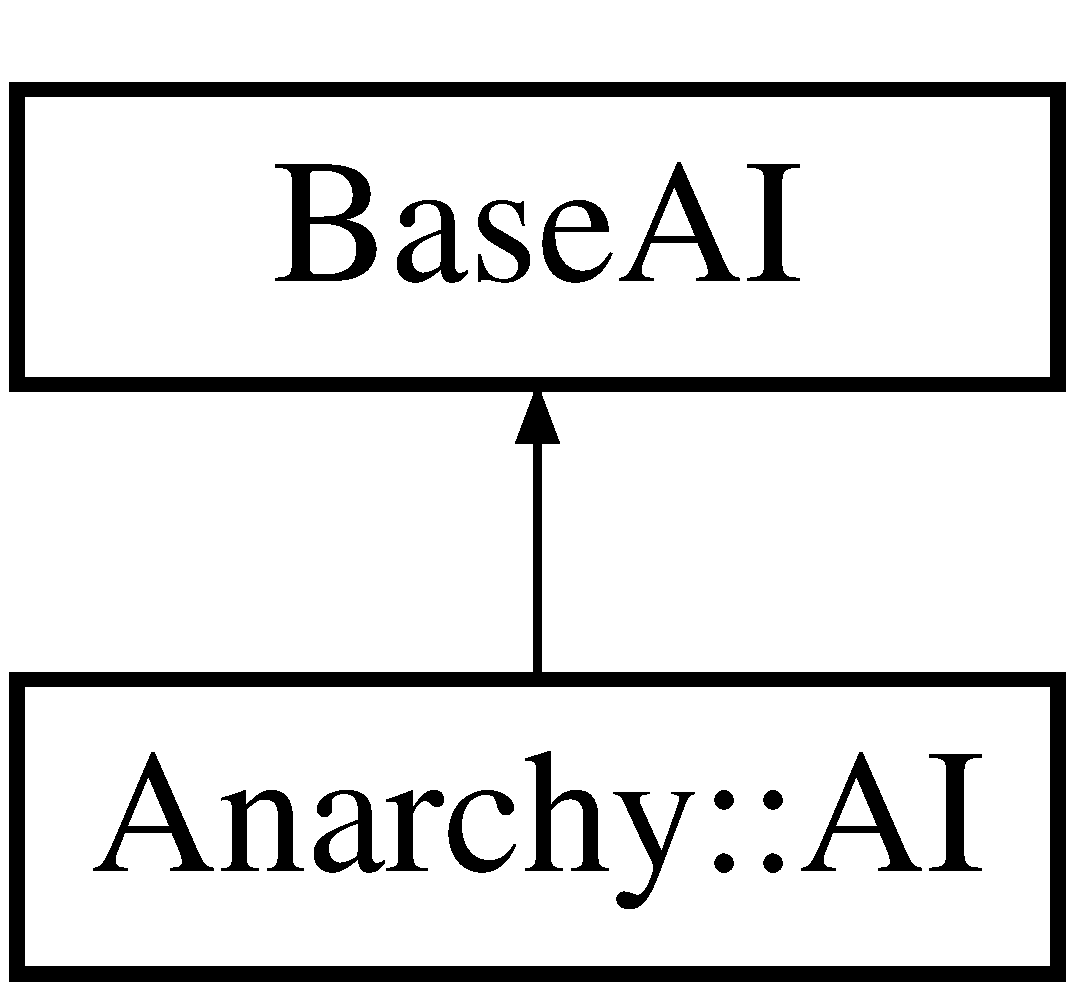
\includegraphics[height=2.000000cm]{classAnarchy_1_1AI}
\end{center}
\end{figure}
\subsection*{Public Member Functions}
\begin{DoxyCompactItemize}
\item 
std\-::string \hyperlink{classAnarchy_1_1AI_a85abf255935e41d562672b9f0ae18161}{get\-Name} ()
\begin{DoxyCompactList}\small\item\em This returns your \hyperlink{classAnarchy_1_1AI}{A\-I}'s name to the game server. Just replace the string. \end{DoxyCompactList}\item 
void \hyperlink{classAnarchy_1_1AI_aa3e5c1b43bfb7e2dd17a281a5344ce66}{start} ()
\begin{DoxyCompactList}\small\item\em This is automatically called when the game first starts, once the \hyperlink{classAnarchy_1_1Game}{Game} object and all Game\-Objects have been initialized, but before any players do anything. \end{DoxyCompactList}\item 
void \hyperlink{classAnarchy_1_1AI_abd80d138a560c8c8e5610cbbb9f7e434}{game\-Updated} ()
\begin{DoxyCompactList}\small\item\em This is automatically called every time the game (or anything in it) updates. \end{DoxyCompactList}\item 
void \hyperlink{classAnarchy_1_1AI_ad97ef7981850e5b0f2af26582746c1b8}{ended} (bool won, std\-::string reason)
\begin{DoxyCompactList}\small\item\em This is automatically called when the game ends. \end{DoxyCompactList}\item 
bool \hyperlink{classAnarchy_1_1AI_a8f4d08c347f19c4c77fe72291b29235c}{run\-Turn} ()
\begin{DoxyCompactList}\small\item\em This is called every time the \hyperlink{classAnarchy_1_1AI}{A\-I} is asked to respond with a command during their turn \end{DoxyCompactList}\item 
\hypertarget{classAnarchy_1_1AI_a7802b3dc7bfde3c4d5f6a0d4f46aae12}{bool {\bfseries can\-Bribe} (const \hyperlink{classAnarchy_1_1Building}{Building} $\ast$to\-Test) const }\label{classAnarchy_1_1AI_a7802b3dc7bfde3c4d5f6a0d4f46aae12}

\end{DoxyCompactItemize}
\subsection*{Public Attributes}
\begin{DoxyCompactItemize}
\item 
\hyperlink{classAnarchy_1_1Game}{Anarchy\-::\-Game} $\ast$ \hyperlink{classAnarchy_1_1AI_a39d2285ba34412f0f81386a2cc2a5805}{game}
\begin{DoxyCompactList}\small\item\em This is a pointer to the \hyperlink{classAnarchy_1_1Game}{Game} object itself, it contains all the information about the current game \end{DoxyCompactList}\item 
\hyperlink{classAnarchy_1_1Player}{Anarchy\-::\-Player} $\ast$ \hyperlink{classAnarchy_1_1AI_ae0cb94906cf11fba26dfb511530bd52e}{player}
\begin{DoxyCompactList}\small\item\em This is a pointer to your \hyperlink{classAnarchy_1_1AI}{A\-I}'s player. This \hyperlink{classAnarchy_1_1AI}{A\-I} class is not a player, but it should command this \hyperlink{classAnarchy_1_1Player}{Player}. \end{DoxyCompactList}\end{DoxyCompactItemize}


\subsection{Detailed Description}
This the header file for where you build your \hyperlink{classAnarchy_1_1AI}{A\-I} for the Anarchy game. 



\subsection{Member Function Documentation}
\hypertarget{classAnarchy_1_1AI_ad97ef7981850e5b0f2af26582746c1b8}{\index{Anarchy\-::\-A\-I@{Anarchy\-::\-A\-I}!ended@{ended}}
\index{ended@{ended}!Anarchy::AI@{Anarchy\-::\-A\-I}}
\subsubsection[{ended}]{\setlength{\rightskip}{0pt plus 5cm}void Anarchy\-::\-A\-I\-::ended (
\begin{DoxyParamCaption}
\item[{bool}]{won, }
\item[{std\-::string}]{reason}
\end{DoxyParamCaption}
)}}\label{classAnarchy_1_1AI_ad97ef7981850e5b0f2af26582746c1b8}


This is automatically called when the game ends. 


\begin{DoxyParams}{Parameters}
{\em won} & true if your player won, false otherwise\\
\hline
{\em reason} & a string explaining why you won or lost\\
\hline
\end{DoxyParams}
\hypertarget{classAnarchy_1_1AI_abd80d138a560c8c8e5610cbbb9f7e434}{\index{Anarchy\-::\-A\-I@{Anarchy\-::\-A\-I}!game\-Updated@{game\-Updated}}
\index{game\-Updated@{game\-Updated}!Anarchy::AI@{Anarchy\-::\-A\-I}}
\subsubsection[{game\-Updated}]{\setlength{\rightskip}{0pt plus 5cm}void Anarchy\-::\-A\-I\-::game\-Updated (
\begin{DoxyParamCaption}
{}
\end{DoxyParamCaption}
)}}\label{classAnarchy_1_1AI_abd80d138a560c8c8e5610cbbb9f7e434}


This is automatically called every time the game (or anything in it) updates. 

\hypertarget{classAnarchy_1_1AI_a85abf255935e41d562672b9f0ae18161}{\index{Anarchy\-::\-A\-I@{Anarchy\-::\-A\-I}!get\-Name@{get\-Name}}
\index{get\-Name@{get\-Name}!Anarchy::AI@{Anarchy\-::\-A\-I}}
\subsubsection[{get\-Name}]{\setlength{\rightskip}{0pt plus 5cm}std\-::string Anarchy\-::\-A\-I\-::get\-Name (
\begin{DoxyParamCaption}
{}
\end{DoxyParamCaption}
)}}\label{classAnarchy_1_1AI_a85abf255935e41d562672b9f0ae18161}


This returns your \hyperlink{classAnarchy_1_1AI}{A\-I}'s name to the game server. Just replace the string. 

\begin{DoxyReturn}{Returns}
string of you \hyperlink{classAnarchy_1_1AI}{A\-I}'s name.
\end{DoxyReturn}
\hypertarget{classAnarchy_1_1AI_a8f4d08c347f19c4c77fe72291b29235c}{\index{Anarchy\-::\-A\-I@{Anarchy\-::\-A\-I}!run\-Turn@{run\-Turn}}
\index{run\-Turn@{run\-Turn}!Anarchy::AI@{Anarchy\-::\-A\-I}}
\subsubsection[{run\-Turn}]{\setlength{\rightskip}{0pt plus 5cm}bool Anarchy\-::\-A\-I\-::run\-Turn (
\begin{DoxyParamCaption}
{}
\end{DoxyParamCaption}
)}}\label{classAnarchy_1_1AI_a8f4d08c347f19c4c77fe72291b29235c}


This is called every time the \hyperlink{classAnarchy_1_1AI}{A\-I} is asked to respond with a command during their turn 

\begin{DoxyReturn}{Returns}
represents if you want to end your turn. true means end the turn, false means to keep your turn going and re-\/call \hyperlink{classAnarchy_1_1AI_a8f4d08c347f19c4c77fe72291b29235c}{run\-Turn()}
\end{DoxyReturn}
\hypertarget{classAnarchy_1_1AI_aa3e5c1b43bfb7e2dd17a281a5344ce66}{\index{Anarchy\-::\-A\-I@{Anarchy\-::\-A\-I}!start@{start}}
\index{start@{start}!Anarchy::AI@{Anarchy\-::\-A\-I}}
\subsubsection[{start}]{\setlength{\rightskip}{0pt plus 5cm}void Anarchy\-::\-A\-I\-::start (
\begin{DoxyParamCaption}
{}
\end{DoxyParamCaption}
)}}\label{classAnarchy_1_1AI_aa3e5c1b43bfb7e2dd17a281a5344ce66}


This is automatically called when the game first starts, once the \hyperlink{classAnarchy_1_1Game}{Game} object and all Game\-Objects have been initialized, but before any players do anything. 



\subsection{Member Data Documentation}
\hypertarget{classAnarchy_1_1AI_a39d2285ba34412f0f81386a2cc2a5805}{\index{Anarchy\-::\-A\-I@{Anarchy\-::\-A\-I}!game@{game}}
\index{game@{game}!Anarchy::AI@{Anarchy\-::\-A\-I}}
\subsubsection[{game}]{\setlength{\rightskip}{0pt plus 5cm}{\bf Anarchy\-::\-Game}$\ast$ Anarchy\-::\-A\-I\-::game}}\label{classAnarchy_1_1AI_a39d2285ba34412f0f81386a2cc2a5805}


This is a pointer to the \hyperlink{classAnarchy_1_1Game}{Game} object itself, it contains all the information about the current game 

\hypertarget{classAnarchy_1_1AI_ae0cb94906cf11fba26dfb511530bd52e}{\index{Anarchy\-::\-A\-I@{Anarchy\-::\-A\-I}!player@{player}}
\index{player@{player}!Anarchy::AI@{Anarchy\-::\-A\-I}}
\subsubsection[{player}]{\setlength{\rightskip}{0pt plus 5cm}{\bf Anarchy\-::\-Player}$\ast$ Anarchy\-::\-A\-I\-::player}}\label{classAnarchy_1_1AI_ae0cb94906cf11fba26dfb511530bd52e}


This is a pointer to your \hyperlink{classAnarchy_1_1AI}{A\-I}'s player. This \hyperlink{classAnarchy_1_1AI}{A\-I} class is not a player, but it should command this \hyperlink{classAnarchy_1_1Player}{Player}. 



The documentation for this class was generated from the following files\-:\begin{DoxyCompactItemize}
\item 
ai.\-h\item 
ai.\-cpp\end{DoxyCompactItemize}

\hypertarget{classAnarchy_1_1Building}{\section{Anarchy\-:\-:Building Class Reference}
\label{classAnarchy_1_1Building}\index{Anarchy\-::\-Building@{Anarchy\-::\-Building}}
}


A basic building. It does nothing besides burn down. Other Buildings inherit from this class.  




{\ttfamily \#include $<$building.\-h$>$}

Inheritance diagram for Anarchy\-:\-:Building\-:\begin{figure}[H]
\begin{center}
\leavevmode
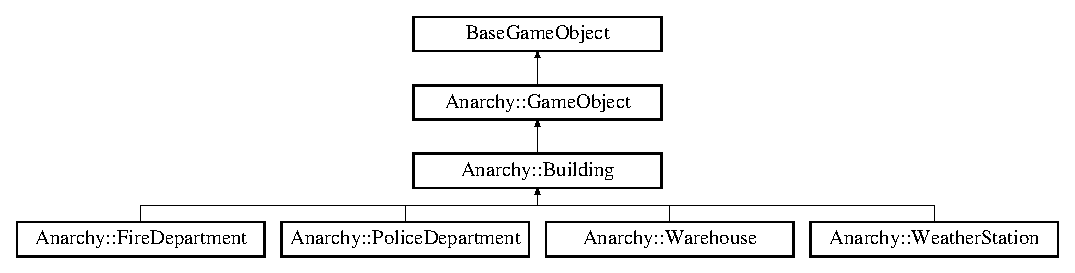
\includegraphics[height=3.218391cm]{classAnarchy_1_1Building}
\end{center}
\end{figure}
\subsection*{Public Attributes}
\begin{DoxyCompactItemize}
\item 
bool \hyperlink{classAnarchy_1_1Building_a2d0079a53d7239ad72be834a168a29a4}{bribed}
\begin{DoxyCompactList}\small\item\em when true this building has already been bribed this turn and cannot be bribed again this turn. \end{DoxyCompactList}\item 
\hyperlink{classAnarchy_1_1Building}{Anarchy\-::\-Building} $\ast$ \hyperlink{classAnarchy_1_1Building_aeecf09082fb73c6b6df35fda22431d79}{building\-East}
\begin{DoxyCompactList}\small\item\em The \hyperlink{classAnarchy_1_1Building}{Building} directly to the east of this building, or null if not present. \end{DoxyCompactList}\item 
\hyperlink{classAnarchy_1_1Building}{Anarchy\-::\-Building} $\ast$ \hyperlink{classAnarchy_1_1Building_aeed7b639ac2199c247d6b168a789acfc}{building\-North}
\begin{DoxyCompactList}\small\item\em The \hyperlink{classAnarchy_1_1Building}{Building} directly to the north of this building, or null if not present. \end{DoxyCompactList}\item 
\hyperlink{classAnarchy_1_1Building}{Anarchy\-::\-Building} $\ast$ \hyperlink{classAnarchy_1_1Building_a12a304929ca4c48f717035b535078c46}{building\-South}
\begin{DoxyCompactList}\small\item\em The \hyperlink{classAnarchy_1_1Building}{Building} directly to the south of this building, or null if not present. \end{DoxyCompactList}\item 
\hyperlink{classAnarchy_1_1Building}{Anarchy\-::\-Building} $\ast$ \hyperlink{classAnarchy_1_1Building_accc6c555aa5cd0e02e88dc727e5fcd79}{building\-West}
\begin{DoxyCompactList}\small\item\em The \hyperlink{classAnarchy_1_1Building}{Building} directly to the west of this building, or null if not present. \end{DoxyCompactList}\item 
int \hyperlink{classAnarchy_1_1Building_a05b636d766c51eba120d9e044d82a402}{fire}
\begin{DoxyCompactList}\small\item\em How much fire is currently burning the building, and thus how much damage it will take at the end of its owner's turn. 0 means no fire. \end{DoxyCompactList}\item 
int \hyperlink{classAnarchy_1_1Building_a3536e925fb8fc11bb403cc0555f935a4}{health}
\begin{DoxyCompactList}\small\item\em How much health this building currently has. When this reaches 0 the \hyperlink{classAnarchy_1_1Building}{Building} has been burned down \end{DoxyCompactList}\item 
bool \hyperlink{classAnarchy_1_1Building_a46e92ca7a40a44b467c58e1c67944d48}{is\-Headquarters}
\begin{DoxyCompactList}\small\item\em true if this is the Headquarters of the owning player, false otherwise. Burning this down wins the game for the other \hyperlink{classAnarchy_1_1Player}{Player}. \end{DoxyCompactList}\item 
\hyperlink{classAnarchy_1_1Player}{Anarchy\-::\-Player} $\ast$ \hyperlink{classAnarchy_1_1Building_ab3e204cfff1707cb86793b7889958e7f}{owner}
\begin{DoxyCompactList}\small\item\em The player that owns this building. If it burns down (health reaches 0) that player gets an additional bribe(s). \end{DoxyCompactList}\item 
int \hyperlink{classAnarchy_1_1Building_a4748629dadd04cc82b3894214c764724}{x}
\begin{DoxyCompactList}\small\item\em The location of the \hyperlink{classAnarchy_1_1Building}{Building} along the x-\/axis \end{DoxyCompactList}\item 
int \hyperlink{classAnarchy_1_1Building_a9f3e61c752dba70cec82fc293444f295}{y}
\begin{DoxyCompactList}\small\item\em The location of the \hyperlink{classAnarchy_1_1Building}{Building} along the y-\/axis \end{DoxyCompactList}\end{DoxyCompactItemize}
\subsection*{Protected Member Functions}
\begin{DoxyCompactItemize}
\item 
\hypertarget{classAnarchy_1_1Building_af5ecbdb03b63bdd2fa38ac599bf74410}{virtual void {\bfseries delta\-Update\-Field} (const std\-::string \&field\-Name, boost\-::property\-\_\-tree\-::ptree \&delta)}\label{classAnarchy_1_1Building_af5ecbdb03b63bdd2fa38ac599bf74410}

\end{DoxyCompactItemize}
\subsection*{Additional Inherited Members}


\subsection{Detailed Description}
A basic building. It does nothing besides burn down. Other Buildings inherit from this class. 



\subsection{Member Data Documentation}
\hypertarget{classAnarchy_1_1Building_a2d0079a53d7239ad72be834a168a29a4}{\index{Anarchy\-::\-Building@{Anarchy\-::\-Building}!bribed@{bribed}}
\index{bribed@{bribed}!Anarchy::Building@{Anarchy\-::\-Building}}
\subsubsection[{bribed}]{\setlength{\rightskip}{0pt plus 5cm}bool Anarchy\-::\-Building\-::bribed}}\label{classAnarchy_1_1Building_a2d0079a53d7239ad72be834a168a29a4}


when true this building has already been bribed this turn and cannot be bribed again this turn. 

\hypertarget{classAnarchy_1_1Building_aeecf09082fb73c6b6df35fda22431d79}{\index{Anarchy\-::\-Building@{Anarchy\-::\-Building}!building\-East@{building\-East}}
\index{building\-East@{building\-East}!Anarchy::Building@{Anarchy\-::\-Building}}
\subsubsection[{building\-East}]{\setlength{\rightskip}{0pt plus 5cm}{\bf Anarchy\-::\-Building}$\ast$ Anarchy\-::\-Building\-::building\-East}}\label{classAnarchy_1_1Building_aeecf09082fb73c6b6df35fda22431d79}


The \hyperlink{classAnarchy_1_1Building}{Building} directly to the east of this building, or null if not present. 

\hypertarget{classAnarchy_1_1Building_aeed7b639ac2199c247d6b168a789acfc}{\index{Anarchy\-::\-Building@{Anarchy\-::\-Building}!building\-North@{building\-North}}
\index{building\-North@{building\-North}!Anarchy::Building@{Anarchy\-::\-Building}}
\subsubsection[{building\-North}]{\setlength{\rightskip}{0pt plus 5cm}{\bf Anarchy\-::\-Building}$\ast$ Anarchy\-::\-Building\-::building\-North}}\label{classAnarchy_1_1Building_aeed7b639ac2199c247d6b168a789acfc}


The \hyperlink{classAnarchy_1_1Building}{Building} directly to the north of this building, or null if not present. 

\hypertarget{classAnarchy_1_1Building_a12a304929ca4c48f717035b535078c46}{\index{Anarchy\-::\-Building@{Anarchy\-::\-Building}!building\-South@{building\-South}}
\index{building\-South@{building\-South}!Anarchy::Building@{Anarchy\-::\-Building}}
\subsubsection[{building\-South}]{\setlength{\rightskip}{0pt plus 5cm}{\bf Anarchy\-::\-Building}$\ast$ Anarchy\-::\-Building\-::building\-South}}\label{classAnarchy_1_1Building_a12a304929ca4c48f717035b535078c46}


The \hyperlink{classAnarchy_1_1Building}{Building} directly to the south of this building, or null if not present. 

\hypertarget{classAnarchy_1_1Building_accc6c555aa5cd0e02e88dc727e5fcd79}{\index{Anarchy\-::\-Building@{Anarchy\-::\-Building}!building\-West@{building\-West}}
\index{building\-West@{building\-West}!Anarchy::Building@{Anarchy\-::\-Building}}
\subsubsection[{building\-West}]{\setlength{\rightskip}{0pt plus 5cm}{\bf Anarchy\-::\-Building}$\ast$ Anarchy\-::\-Building\-::building\-West}}\label{classAnarchy_1_1Building_accc6c555aa5cd0e02e88dc727e5fcd79}


The \hyperlink{classAnarchy_1_1Building}{Building} directly to the west of this building, or null if not present. 

\hypertarget{classAnarchy_1_1Building_a05b636d766c51eba120d9e044d82a402}{\index{Anarchy\-::\-Building@{Anarchy\-::\-Building}!fire@{fire}}
\index{fire@{fire}!Anarchy::Building@{Anarchy\-::\-Building}}
\subsubsection[{fire}]{\setlength{\rightskip}{0pt plus 5cm}int Anarchy\-::\-Building\-::fire}}\label{classAnarchy_1_1Building_a05b636d766c51eba120d9e044d82a402}


How much fire is currently burning the building, and thus how much damage it will take at the end of its owner's turn. 0 means no fire. 

\hypertarget{classAnarchy_1_1Building_a3536e925fb8fc11bb403cc0555f935a4}{\index{Anarchy\-::\-Building@{Anarchy\-::\-Building}!health@{health}}
\index{health@{health}!Anarchy::Building@{Anarchy\-::\-Building}}
\subsubsection[{health}]{\setlength{\rightskip}{0pt plus 5cm}int Anarchy\-::\-Building\-::health}}\label{classAnarchy_1_1Building_a3536e925fb8fc11bb403cc0555f935a4}


How much health this building currently has. When this reaches 0 the \hyperlink{classAnarchy_1_1Building}{Building} has been burned down 

\hypertarget{classAnarchy_1_1Building_a46e92ca7a40a44b467c58e1c67944d48}{\index{Anarchy\-::\-Building@{Anarchy\-::\-Building}!is\-Headquarters@{is\-Headquarters}}
\index{is\-Headquarters@{is\-Headquarters}!Anarchy::Building@{Anarchy\-::\-Building}}
\subsubsection[{is\-Headquarters}]{\setlength{\rightskip}{0pt plus 5cm}bool Anarchy\-::\-Building\-::is\-Headquarters}}\label{classAnarchy_1_1Building_a46e92ca7a40a44b467c58e1c67944d48}


true if this is the Headquarters of the owning player, false otherwise. Burning this down wins the game for the other \hyperlink{classAnarchy_1_1Player}{Player}. 

\hypertarget{classAnarchy_1_1Building_ab3e204cfff1707cb86793b7889958e7f}{\index{Anarchy\-::\-Building@{Anarchy\-::\-Building}!owner@{owner}}
\index{owner@{owner}!Anarchy::Building@{Anarchy\-::\-Building}}
\subsubsection[{owner}]{\setlength{\rightskip}{0pt plus 5cm}{\bf Anarchy\-::\-Player}$\ast$ Anarchy\-::\-Building\-::owner}}\label{classAnarchy_1_1Building_ab3e204cfff1707cb86793b7889958e7f}


The player that owns this building. If it burns down (health reaches 0) that player gets an additional bribe(s). 

\hypertarget{classAnarchy_1_1Building_a4748629dadd04cc82b3894214c764724}{\index{Anarchy\-::\-Building@{Anarchy\-::\-Building}!x@{x}}
\index{x@{x}!Anarchy::Building@{Anarchy\-::\-Building}}
\subsubsection[{x}]{\setlength{\rightskip}{0pt plus 5cm}int Anarchy\-::\-Building\-::x}}\label{classAnarchy_1_1Building_a4748629dadd04cc82b3894214c764724}


The location of the \hyperlink{classAnarchy_1_1Building}{Building} along the x-\/axis 

\hypertarget{classAnarchy_1_1Building_a9f3e61c752dba70cec82fc293444f295}{\index{Anarchy\-::\-Building@{Anarchy\-::\-Building}!y@{y}}
\index{y@{y}!Anarchy::Building@{Anarchy\-::\-Building}}
\subsubsection[{y}]{\setlength{\rightskip}{0pt plus 5cm}int Anarchy\-::\-Building\-::y}}\label{classAnarchy_1_1Building_a9f3e61c752dba70cec82fc293444f295}


The location of the \hyperlink{classAnarchy_1_1Building}{Building} along the y-\/axis 



The documentation for this class was generated from the following files\-:\begin{DoxyCompactItemize}
\item 
building.\-h\item 
building.\-cpp\end{DoxyCompactItemize}

\hypertarget{classAnarchy_1_1FireDepartment}{\section{Anarchy\-:\-:Fire\-Department Class Reference}
\label{classAnarchy_1_1FireDepartment}\index{Anarchy\-::\-Fire\-Department@{Anarchy\-::\-Fire\-Department}}
}


Can put out fires completely.  




{\ttfamily \#include $<$fire\-Department.\-h$>$}

Inheritance diagram for Anarchy\-:\-:Fire\-Department\-:\begin{figure}[H]
\begin{center}
\leavevmode
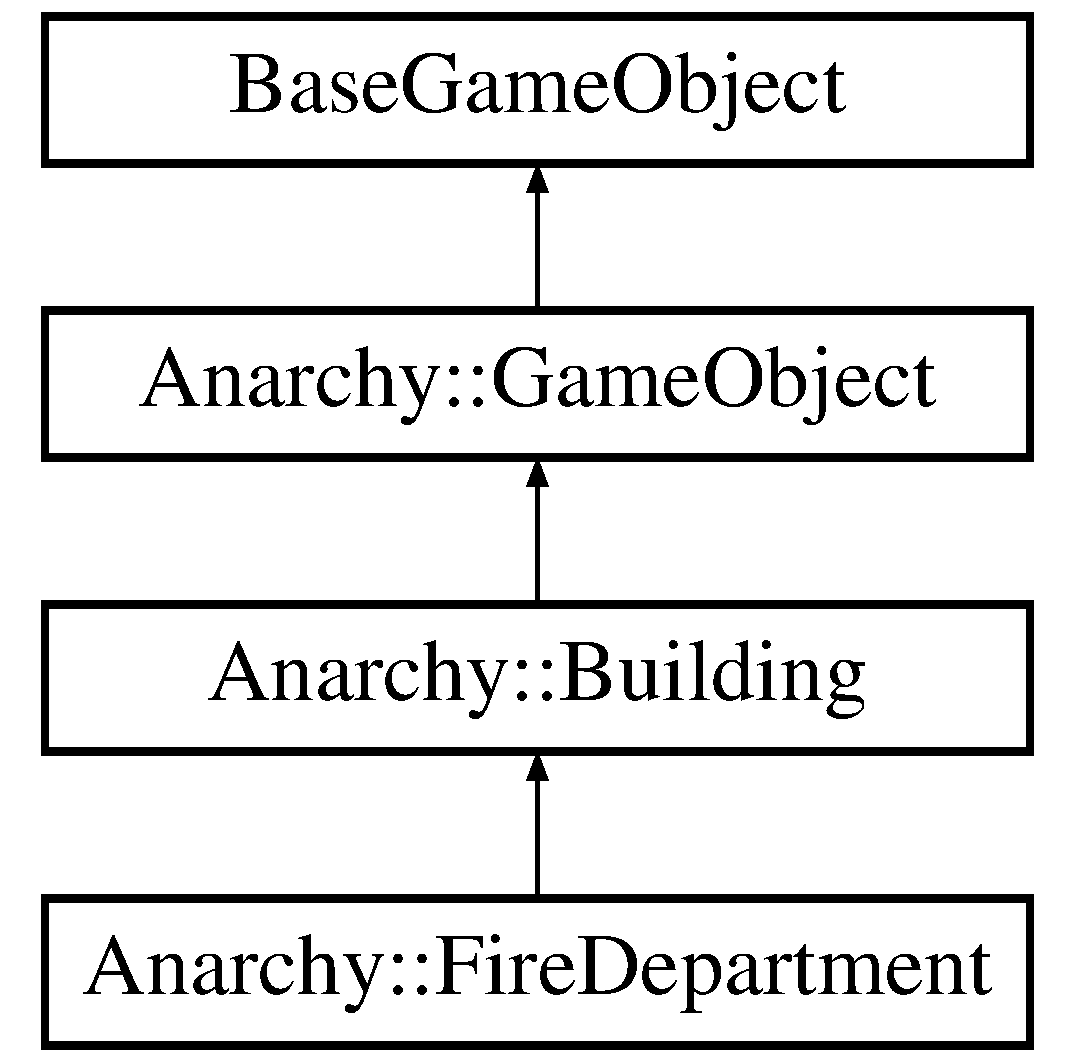
\includegraphics[height=4.000000cm]{classAnarchy_1_1FireDepartment}
\end{center}
\end{figure}
\subsection*{Public Member Functions}
\begin{DoxyCompactItemize}
\item 
bool \hyperlink{classAnarchy_1_1FireDepartment_a0d01ce6fc38d520fa6e6ff4f6b2f134b}{extinguish} (\hyperlink{classAnarchy_1_1Building}{Anarchy\-::\-Building} $\ast$building)
\begin{DoxyCompactList}\small\item\em Bribes this \hyperlink{classAnarchy_1_1FireDepartment}{Fire\-Department} to extinguish the some of the fire in a building. \end{DoxyCompactList}\end{DoxyCompactItemize}
\subsection*{Public Attributes}
\begin{DoxyCompactItemize}
\item 
int \hyperlink{classAnarchy_1_1FireDepartment_a859e81aeb1067f5218d9e894d98bceec}{fire\-Extinguished}
\begin{DoxyCompactList}\small\item\em The amount of fire removed from a building when bribed to extinguish a building. \end{DoxyCompactList}\end{DoxyCompactItemize}
\subsection*{Protected Member Functions}
\begin{DoxyCompactItemize}
\item 
\hypertarget{classAnarchy_1_1FireDepartment_a47726fa7b43561d54237a9c730592ce5}{virtual void {\bfseries delta\-Update\-Field} (const std\-::string \&field\-Name, boost\-::property\-\_\-tree\-::ptree \&delta)}\label{classAnarchy_1_1FireDepartment_a47726fa7b43561d54237a9c730592ce5}

\end{DoxyCompactItemize}


\subsection{Detailed Description}
Can put out fires completely. 



\subsection{Member Function Documentation}
\hypertarget{classAnarchy_1_1FireDepartment_a0d01ce6fc38d520fa6e6ff4f6b2f134b}{\index{Anarchy\-::\-Fire\-Department@{Anarchy\-::\-Fire\-Department}!extinguish@{extinguish}}
\index{extinguish@{extinguish}!Anarchy::FireDepartment@{Anarchy\-::\-Fire\-Department}}
\subsubsection[{extinguish}]{\setlength{\rightskip}{0pt plus 5cm}bool Anarchy\-::\-Fire\-Department\-::extinguish (
\begin{DoxyParamCaption}
\item[{{\bf Anarchy\-::\-Building} $\ast$}]{building}
\end{DoxyParamCaption}
)}}\label{classAnarchy_1_1FireDepartment_a0d01ce6fc38d520fa6e6ff4f6b2f134b}


Bribes this \hyperlink{classAnarchy_1_1FireDepartment}{Fire\-Department} to extinguish the some of the fire in a building. 


\begin{DoxyParams}{Parameters}
{\em building} & The \hyperlink{classAnarchy_1_1Building}{Building} you want to extinguish.\\
\hline
\end{DoxyParams}
\begin{DoxyReturn}{Returns}
true if the bribe worked, false otherwise
\end{DoxyReturn}


\subsection{Member Data Documentation}
\hypertarget{classAnarchy_1_1FireDepartment_a859e81aeb1067f5218d9e894d98bceec}{\index{Anarchy\-::\-Fire\-Department@{Anarchy\-::\-Fire\-Department}!fire\-Extinguished@{fire\-Extinguished}}
\index{fire\-Extinguished@{fire\-Extinguished}!Anarchy::FireDepartment@{Anarchy\-::\-Fire\-Department}}
\subsubsection[{fire\-Extinguished}]{\setlength{\rightskip}{0pt plus 5cm}int Anarchy\-::\-Fire\-Department\-::fire\-Extinguished}}\label{classAnarchy_1_1FireDepartment_a859e81aeb1067f5218d9e894d98bceec}


The amount of fire removed from a building when bribed to extinguish a building. 



The documentation for this class was generated from the following files\-:\begin{DoxyCompactItemize}
\item 
fire\-Department.\-h\item 
fire\-Department.\-cpp\end{DoxyCompactItemize}

\hypertarget{classAnarchy_1_1Forecast}{\section{Anarchy\-:\-:Forecast Class Reference}
\label{classAnarchy_1_1Forecast}\index{Anarchy\-::\-Forecast@{Anarchy\-::\-Forecast}}
}


The weather effect that will be applied at the end of a turn, which causes fires to spread.  




{\ttfamily \#include $<$forecast.\-h$>$}

Inheritance diagram for Anarchy\-:\-:Forecast\-:\begin{figure}[H]
\begin{center}
\leavevmode
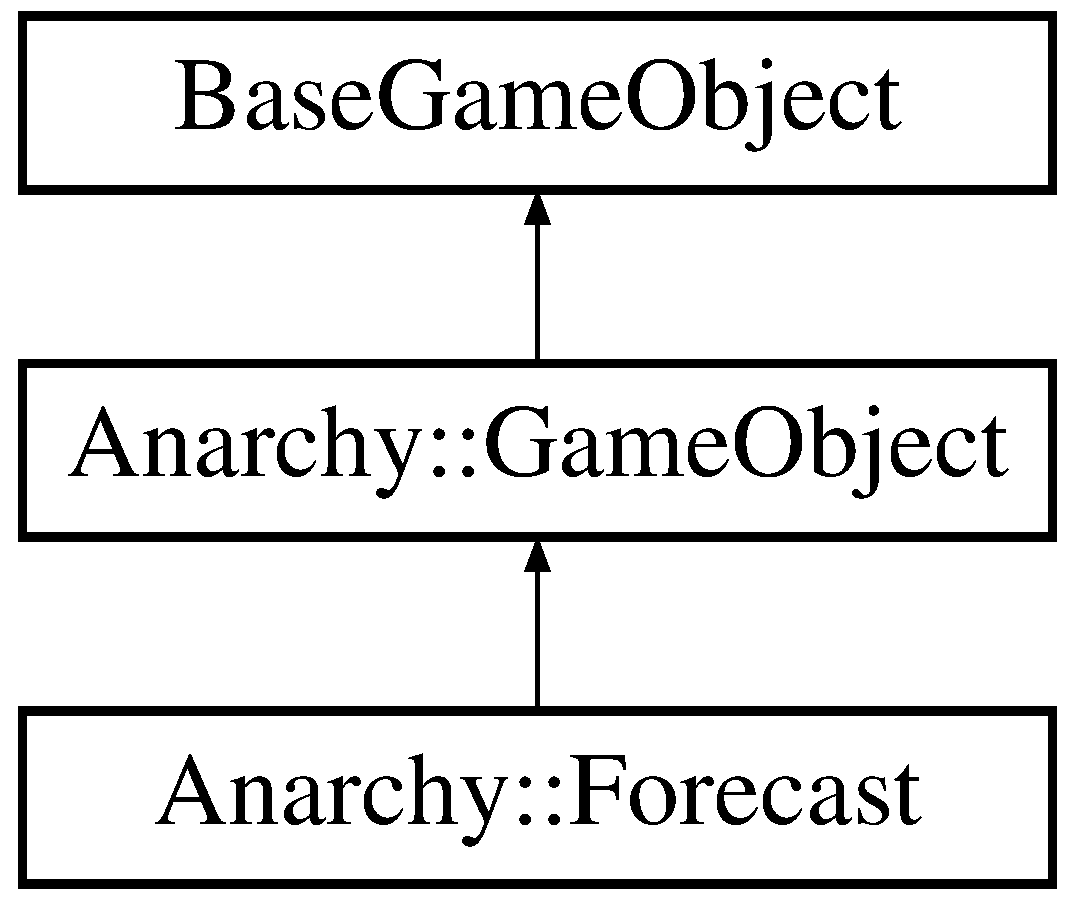
\includegraphics[height=3.000000cm]{classAnarchy_1_1Forecast}
\end{center}
\end{figure}
\subsection*{Public Attributes}
\begin{DoxyCompactItemize}
\item 
\hyperlink{classAnarchy_1_1Player}{Anarchy\-::\-Player} $\ast$ \hyperlink{classAnarchy_1_1Forecast_a3e6c133fea0591d299943a5e3216211d}{controlling\-Player}
\begin{DoxyCompactList}\small\item\em The \hyperlink{classAnarchy_1_1Player}{Player} that can use Weather\-Stations to control this \hyperlink{classAnarchy_1_1Forecast}{Forecast} when its the next\-Forecast. \end{DoxyCompactList}\item 
std\-::string \hyperlink{classAnarchy_1_1Forecast_ae1e9bbacab6d18bbec3cbb0e5a33756b}{direction}
\begin{DoxyCompactList}\small\item\em The direction the wind will blow fires in. Can be 'north', 'east', 'south', or 'west' \end{DoxyCompactList}\item 
int \hyperlink{classAnarchy_1_1Forecast_a18d05c207ab1e31e06ecdc5781f50499}{intensity}
\begin{DoxyCompactList}\small\item\em How much of a \hyperlink{classAnarchy_1_1Building}{Building}'s fire that can be blown in the direction of this \hyperlink{classAnarchy_1_1Forecast}{Forecast}. Fire is duplicated (copied), not moved (transfered). \end{DoxyCompactList}\end{DoxyCompactItemize}
\subsection*{Protected Member Functions}
\begin{DoxyCompactItemize}
\item 
\hypertarget{classAnarchy_1_1Forecast_a231e15518a6467e6237a6eb55ca50c8a}{virtual void {\bfseries delta\-Update\-Field} (const std\-::string \&field\-Name, boost\-::property\-\_\-tree\-::ptree \&delta)}\label{classAnarchy_1_1Forecast_a231e15518a6467e6237a6eb55ca50c8a}

\end{DoxyCompactItemize}
\subsection*{Additional Inherited Members}


\subsection{Detailed Description}
The weather effect that will be applied at the end of a turn, which causes fires to spread. 



\subsection{Member Data Documentation}
\hypertarget{classAnarchy_1_1Forecast_a3e6c133fea0591d299943a5e3216211d}{\index{Anarchy\-::\-Forecast@{Anarchy\-::\-Forecast}!controlling\-Player@{controlling\-Player}}
\index{controlling\-Player@{controlling\-Player}!Anarchy::Forecast@{Anarchy\-::\-Forecast}}
\subsubsection[{controlling\-Player}]{\setlength{\rightskip}{0pt plus 5cm}{\bf Anarchy\-::\-Player}$\ast$ Anarchy\-::\-Forecast\-::controlling\-Player}}\label{classAnarchy_1_1Forecast_a3e6c133fea0591d299943a5e3216211d}


The \hyperlink{classAnarchy_1_1Player}{Player} that can use Weather\-Stations to control this \hyperlink{classAnarchy_1_1Forecast}{Forecast} when its the next\-Forecast. 

\hypertarget{classAnarchy_1_1Forecast_ae1e9bbacab6d18bbec3cbb0e5a33756b}{\index{Anarchy\-::\-Forecast@{Anarchy\-::\-Forecast}!direction@{direction}}
\index{direction@{direction}!Anarchy::Forecast@{Anarchy\-::\-Forecast}}
\subsubsection[{direction}]{\setlength{\rightskip}{0pt plus 5cm}std\-::string Anarchy\-::\-Forecast\-::direction}}\label{classAnarchy_1_1Forecast_ae1e9bbacab6d18bbec3cbb0e5a33756b}


The direction the wind will blow fires in. Can be 'north', 'east', 'south', or 'west' 

\hypertarget{classAnarchy_1_1Forecast_a18d05c207ab1e31e06ecdc5781f50499}{\index{Anarchy\-::\-Forecast@{Anarchy\-::\-Forecast}!intensity@{intensity}}
\index{intensity@{intensity}!Anarchy::Forecast@{Anarchy\-::\-Forecast}}
\subsubsection[{intensity}]{\setlength{\rightskip}{0pt plus 5cm}int Anarchy\-::\-Forecast\-::intensity}}\label{classAnarchy_1_1Forecast_a18d05c207ab1e31e06ecdc5781f50499}


How much of a \hyperlink{classAnarchy_1_1Building}{Building}'s fire that can be blown in the direction of this \hyperlink{classAnarchy_1_1Forecast}{Forecast}. Fire is duplicated (copied), not moved (transfered). 



The documentation for this class was generated from the following files\-:\begin{DoxyCompactItemize}
\item 
forecast.\-h\item 
forecast.\-cpp\end{DoxyCompactItemize}

\hypertarget{classAnarchy_1_1Game}{\section{Anarchy\-:\-:Game Class Reference}
\label{classAnarchy_1_1Game}\index{Anarchy\-::\-Game@{Anarchy\-::\-Game}}
}


Two player grid based game where each player tries to burn down the other player's buildings. Let it burn!  




{\ttfamily \#include $<$game.\-h$>$}

Inheritance diagram for Anarchy\-:\-:Game\-:\begin{figure}[H]
\begin{center}
\leavevmode
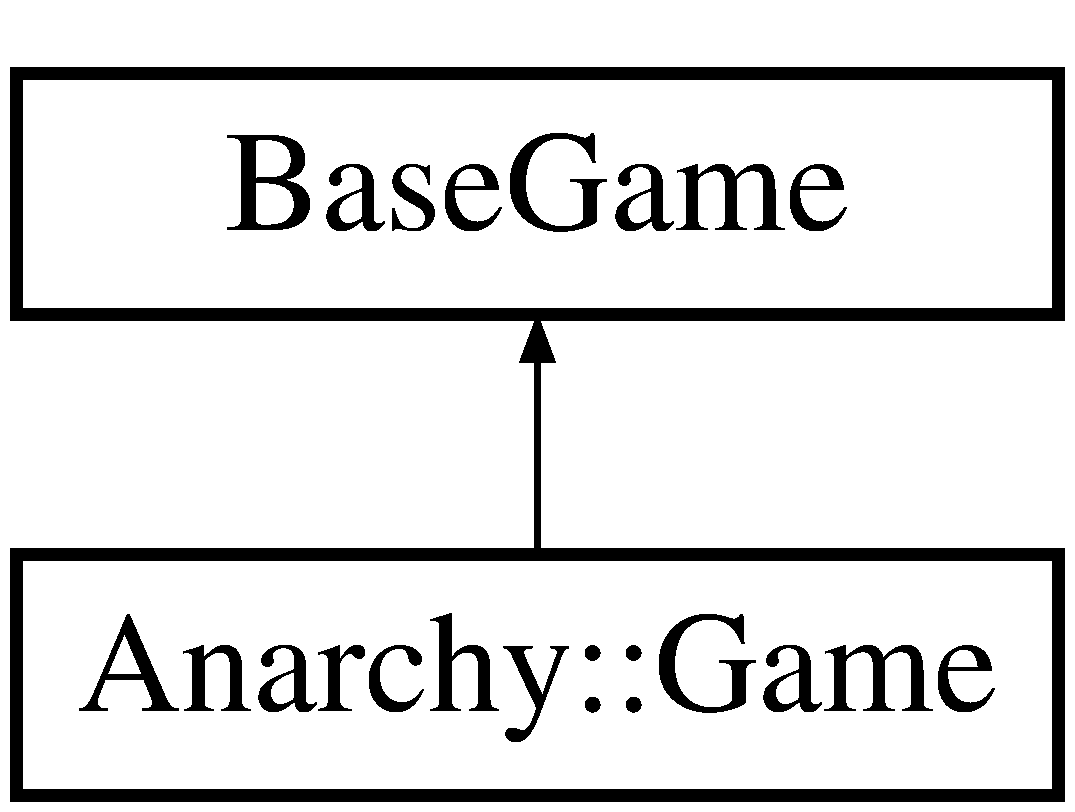
\includegraphics[height=2.000000cm]{classAnarchy_1_1Game}
\end{center}
\end{figure}
\subsection*{Public Attributes}
\begin{DoxyCompactItemize}
\item 
int \hyperlink{classAnarchy_1_1Game_a32c7550663b124a3c3f9f854d0ed0a72}{base\-Bribes\-Per\-Turn}
\begin{DoxyCompactList}\small\item\em How many bribes players get at the beginning of their turn, not counting their burned down Buildings. \end{DoxyCompactList}\item 
std\-::vector$<$ \hyperlink{classAnarchy_1_1Building}{Anarchy\-::\-Building} $\ast$ $>$ \hyperlink{classAnarchy_1_1Game_afed9b69dccd790514505d662b84d5573}{buildings}
\begin{DoxyCompactList}\small\item\em All the buildings in the game. \end{DoxyCompactList}\item 
\hyperlink{classAnarchy_1_1Forecast}{Anarchy\-::\-Forecast} $\ast$ \hyperlink{classAnarchy_1_1Game_a4429e9c4a6613416867b241c37616562}{current\-Forecast}
\begin{DoxyCompactList}\small\item\em The current \hyperlink{classAnarchy_1_1Forecast}{Forecast}, which will be applied at the end of the turn. \end{DoxyCompactList}\item 
\hyperlink{classAnarchy_1_1Player}{Anarchy\-::\-Player} $\ast$ \hyperlink{classAnarchy_1_1Game_ab9c7ef6e3dc9841ebfd6e30423d31677}{current\-Player}
\begin{DoxyCompactList}\small\item\em The player whose turn it is currently. That player can send commands. Other players cannot. \end{DoxyCompactList}\item 
int \hyperlink{classAnarchy_1_1Game_a5ce8941697b3ca1e33d4a98b33a9c797}{current\-Turn}
\begin{DoxyCompactList}\small\item\em The current turn number, starting at 0 for the first player's turn \end{DoxyCompactList}\item 
std\-::vector$<$ \hyperlink{classAnarchy_1_1Forecast}{Anarchy\-::\-Forecast} $\ast$ $>$ \hyperlink{classAnarchy_1_1Game_a756081a4d3d50cc285d0fac27eea7c5d}{forecasts}
\begin{DoxyCompactList}\small\item\em All the forecasts in the game, indexed by turn number. \end{DoxyCompactList}\item 
int \hyperlink{classAnarchy_1_1Game_aaa29aba3235be8bcd5103507ce42b423}{map\-Height}
\begin{DoxyCompactList}\small\item\em The width of the entire map along the vertical (y) axis. \end{DoxyCompactList}\item 
int \hyperlink{classAnarchy_1_1Game_a7693a0b5c342b32fda1de11b1b03d541}{map\-Width}
\begin{DoxyCompactList}\small\item\em The width of the entire map along the horizontal (x) axis. \end{DoxyCompactList}\item 
int \hyperlink{classAnarchy_1_1Game_a306fca75bb8c449f1e17a1ec38c2ab97}{max\-Fire}
\begin{DoxyCompactList}\small\item\em The maximum amount of fire value for any \hyperlink{classAnarchy_1_1Building}{Building}. \end{DoxyCompactList}\item 
int \hyperlink{classAnarchy_1_1Game_a6565f400e8dcdeecb5466a76f3da9beb}{max\-Forecast\-Intensity}
\begin{DoxyCompactList}\small\item\em The maximum amount of intensity value for any \hyperlink{classAnarchy_1_1Forecast}{Forecast}. \end{DoxyCompactList}\item 
int \hyperlink{classAnarchy_1_1Game_a47e287119862163ec1bd33f0f5be15c0}{max\-Turns}
\begin{DoxyCompactList}\small\item\em The maximum number of turns before the game will automatically end. \end{DoxyCompactList}\item 
\hyperlink{classAnarchy_1_1Forecast}{Anarchy\-::\-Forecast} $\ast$ \hyperlink{classAnarchy_1_1Game_ab5709ad48347f087ca94fc6912be6da3}{next\-Forecast}
\begin{DoxyCompactList}\small\item\em The next \hyperlink{classAnarchy_1_1Forecast}{Forecast}, which will be applied at the end of your opponent's turn. This is also the \hyperlink{classAnarchy_1_1Forecast}{Forecast} Weather\-Stations can control this turn. \end{DoxyCompactList}\item 
std\-::vector$<$ \hyperlink{classAnarchy_1_1Player}{Anarchy\-::\-Player} $\ast$ $>$ \hyperlink{classAnarchy_1_1Game_a7320fea6bc1ac442a31ec2b96dd9eee8}{players}
\begin{DoxyCompactList}\small\item\em List of all the players in the game. \end{DoxyCompactList}\item 
std\-::string \hyperlink{classAnarchy_1_1Game_a575c3471b0f8813e00559d0f85d37cf1}{session}
\begin{DoxyCompactList}\small\item\em A unique identifier for the game instance that is being played. \end{DoxyCompactList}\end{DoxyCompactItemize}
\subsection*{Protected Member Functions}
\begin{DoxyCompactItemize}
\item 
\hypertarget{classAnarchy_1_1Game_a10996ad01e194463698355ec39a4328e}{virtual void {\bfseries delta\-Update\-Field} (const std\-::string \&field\-Name, boost\-::property\-\_\-tree\-::ptree \&delta)}\label{classAnarchy_1_1Game_a10996ad01e194463698355ec39a4328e}

\end{DoxyCompactItemize}


\subsection{Detailed Description}
Two player grid based game where each player tries to burn down the other player's buildings. Let it burn! 



\subsection{Member Data Documentation}
\hypertarget{classAnarchy_1_1Game_a32c7550663b124a3c3f9f854d0ed0a72}{\index{Anarchy\-::\-Game@{Anarchy\-::\-Game}!base\-Bribes\-Per\-Turn@{base\-Bribes\-Per\-Turn}}
\index{base\-Bribes\-Per\-Turn@{base\-Bribes\-Per\-Turn}!Anarchy::Game@{Anarchy\-::\-Game}}
\subsubsection[{base\-Bribes\-Per\-Turn}]{\setlength{\rightskip}{0pt plus 5cm}int Anarchy\-::\-Game\-::base\-Bribes\-Per\-Turn}}\label{classAnarchy_1_1Game_a32c7550663b124a3c3f9f854d0ed0a72}


How many bribes players get at the beginning of their turn, not counting their burned down Buildings. 

\hypertarget{classAnarchy_1_1Game_afed9b69dccd790514505d662b84d5573}{\index{Anarchy\-::\-Game@{Anarchy\-::\-Game}!buildings@{buildings}}
\index{buildings@{buildings}!Anarchy::Game@{Anarchy\-::\-Game}}
\subsubsection[{buildings}]{\setlength{\rightskip}{0pt plus 5cm}std\-::vector$<${\bf Anarchy\-::\-Building}$\ast$$>$ Anarchy\-::\-Game\-::buildings}}\label{classAnarchy_1_1Game_afed9b69dccd790514505d662b84d5573}


All the buildings in the game. 

\hypertarget{classAnarchy_1_1Game_a4429e9c4a6613416867b241c37616562}{\index{Anarchy\-::\-Game@{Anarchy\-::\-Game}!current\-Forecast@{current\-Forecast}}
\index{current\-Forecast@{current\-Forecast}!Anarchy::Game@{Anarchy\-::\-Game}}
\subsubsection[{current\-Forecast}]{\setlength{\rightskip}{0pt plus 5cm}{\bf Anarchy\-::\-Forecast}$\ast$ Anarchy\-::\-Game\-::current\-Forecast}}\label{classAnarchy_1_1Game_a4429e9c4a6613416867b241c37616562}


The current \hyperlink{classAnarchy_1_1Forecast}{Forecast}, which will be applied at the end of the turn. 

\hypertarget{classAnarchy_1_1Game_ab9c7ef6e3dc9841ebfd6e30423d31677}{\index{Anarchy\-::\-Game@{Anarchy\-::\-Game}!current\-Player@{current\-Player}}
\index{current\-Player@{current\-Player}!Anarchy::Game@{Anarchy\-::\-Game}}
\subsubsection[{current\-Player}]{\setlength{\rightskip}{0pt plus 5cm}{\bf Anarchy\-::\-Player}$\ast$ Anarchy\-::\-Game\-::current\-Player}}\label{classAnarchy_1_1Game_ab9c7ef6e3dc9841ebfd6e30423d31677}


The player whose turn it is currently. That player can send commands. Other players cannot. 

\hypertarget{classAnarchy_1_1Game_a5ce8941697b3ca1e33d4a98b33a9c797}{\index{Anarchy\-::\-Game@{Anarchy\-::\-Game}!current\-Turn@{current\-Turn}}
\index{current\-Turn@{current\-Turn}!Anarchy::Game@{Anarchy\-::\-Game}}
\subsubsection[{current\-Turn}]{\setlength{\rightskip}{0pt plus 5cm}int Anarchy\-::\-Game\-::current\-Turn}}\label{classAnarchy_1_1Game_a5ce8941697b3ca1e33d4a98b33a9c797}


The current turn number, starting at 0 for the first player's turn 

\hypertarget{classAnarchy_1_1Game_a756081a4d3d50cc285d0fac27eea7c5d}{\index{Anarchy\-::\-Game@{Anarchy\-::\-Game}!forecasts@{forecasts}}
\index{forecasts@{forecasts}!Anarchy::Game@{Anarchy\-::\-Game}}
\subsubsection[{forecasts}]{\setlength{\rightskip}{0pt plus 5cm}std\-::vector$<${\bf Anarchy\-::\-Forecast}$\ast$$>$ Anarchy\-::\-Game\-::forecasts}}\label{classAnarchy_1_1Game_a756081a4d3d50cc285d0fac27eea7c5d}


All the forecasts in the game, indexed by turn number. 

\hypertarget{classAnarchy_1_1Game_aaa29aba3235be8bcd5103507ce42b423}{\index{Anarchy\-::\-Game@{Anarchy\-::\-Game}!map\-Height@{map\-Height}}
\index{map\-Height@{map\-Height}!Anarchy::Game@{Anarchy\-::\-Game}}
\subsubsection[{map\-Height}]{\setlength{\rightskip}{0pt plus 5cm}int Anarchy\-::\-Game\-::map\-Height}}\label{classAnarchy_1_1Game_aaa29aba3235be8bcd5103507ce42b423}


The width of the entire map along the vertical (y) axis. 

\hypertarget{classAnarchy_1_1Game_a7693a0b5c342b32fda1de11b1b03d541}{\index{Anarchy\-::\-Game@{Anarchy\-::\-Game}!map\-Width@{map\-Width}}
\index{map\-Width@{map\-Width}!Anarchy::Game@{Anarchy\-::\-Game}}
\subsubsection[{map\-Width}]{\setlength{\rightskip}{0pt plus 5cm}int Anarchy\-::\-Game\-::map\-Width}}\label{classAnarchy_1_1Game_a7693a0b5c342b32fda1de11b1b03d541}


The width of the entire map along the horizontal (x) axis. 

\hypertarget{classAnarchy_1_1Game_a306fca75bb8c449f1e17a1ec38c2ab97}{\index{Anarchy\-::\-Game@{Anarchy\-::\-Game}!max\-Fire@{max\-Fire}}
\index{max\-Fire@{max\-Fire}!Anarchy::Game@{Anarchy\-::\-Game}}
\subsubsection[{max\-Fire}]{\setlength{\rightskip}{0pt plus 5cm}int Anarchy\-::\-Game\-::max\-Fire}}\label{classAnarchy_1_1Game_a306fca75bb8c449f1e17a1ec38c2ab97}


The maximum amount of fire value for any \hyperlink{classAnarchy_1_1Building}{Building}. 

\hypertarget{classAnarchy_1_1Game_a6565f400e8dcdeecb5466a76f3da9beb}{\index{Anarchy\-::\-Game@{Anarchy\-::\-Game}!max\-Forecast\-Intensity@{max\-Forecast\-Intensity}}
\index{max\-Forecast\-Intensity@{max\-Forecast\-Intensity}!Anarchy::Game@{Anarchy\-::\-Game}}
\subsubsection[{max\-Forecast\-Intensity}]{\setlength{\rightskip}{0pt plus 5cm}int Anarchy\-::\-Game\-::max\-Forecast\-Intensity}}\label{classAnarchy_1_1Game_a6565f400e8dcdeecb5466a76f3da9beb}


The maximum amount of intensity value for any \hyperlink{classAnarchy_1_1Forecast}{Forecast}. 

\hypertarget{classAnarchy_1_1Game_a47e287119862163ec1bd33f0f5be15c0}{\index{Anarchy\-::\-Game@{Anarchy\-::\-Game}!max\-Turns@{max\-Turns}}
\index{max\-Turns@{max\-Turns}!Anarchy::Game@{Anarchy\-::\-Game}}
\subsubsection[{max\-Turns}]{\setlength{\rightskip}{0pt plus 5cm}int Anarchy\-::\-Game\-::max\-Turns}}\label{classAnarchy_1_1Game_a47e287119862163ec1bd33f0f5be15c0}


The maximum number of turns before the game will automatically end. 

\hypertarget{classAnarchy_1_1Game_ab5709ad48347f087ca94fc6912be6da3}{\index{Anarchy\-::\-Game@{Anarchy\-::\-Game}!next\-Forecast@{next\-Forecast}}
\index{next\-Forecast@{next\-Forecast}!Anarchy::Game@{Anarchy\-::\-Game}}
\subsubsection[{next\-Forecast}]{\setlength{\rightskip}{0pt plus 5cm}{\bf Anarchy\-::\-Forecast}$\ast$ Anarchy\-::\-Game\-::next\-Forecast}}\label{classAnarchy_1_1Game_ab5709ad48347f087ca94fc6912be6da3}


The next \hyperlink{classAnarchy_1_1Forecast}{Forecast}, which will be applied at the end of your opponent's turn. This is also the \hyperlink{classAnarchy_1_1Forecast}{Forecast} Weather\-Stations can control this turn. 

\hypertarget{classAnarchy_1_1Game_a7320fea6bc1ac442a31ec2b96dd9eee8}{\index{Anarchy\-::\-Game@{Anarchy\-::\-Game}!players@{players}}
\index{players@{players}!Anarchy::Game@{Anarchy\-::\-Game}}
\subsubsection[{players}]{\setlength{\rightskip}{0pt plus 5cm}std\-::vector$<${\bf Anarchy\-::\-Player}$\ast$$>$ Anarchy\-::\-Game\-::players}}\label{classAnarchy_1_1Game_a7320fea6bc1ac442a31ec2b96dd9eee8}


List of all the players in the game. 

\hypertarget{classAnarchy_1_1Game_a575c3471b0f8813e00559d0f85d37cf1}{\index{Anarchy\-::\-Game@{Anarchy\-::\-Game}!session@{session}}
\index{session@{session}!Anarchy::Game@{Anarchy\-::\-Game}}
\subsubsection[{session}]{\setlength{\rightskip}{0pt plus 5cm}std\-::string Anarchy\-::\-Game\-::session}}\label{classAnarchy_1_1Game_a575c3471b0f8813e00559d0f85d37cf1}


A unique identifier for the game instance that is being played. 



The documentation for this class was generated from the following files\-:\begin{DoxyCompactItemize}
\item 
game.\-h\item 
game.\-cpp\end{DoxyCompactItemize}

\hypertarget{classAnarchy_1_1GameManager}{\section{Anarchy\-:\-:Game\-Manager Class Reference}
\label{classAnarchy_1_1GameManager}\index{Anarchy\-::\-Game\-Manager@{Anarchy\-::\-Game\-Manager}}
}


This is a class that manages the Anarchy \hyperlink{classAnarchy_1_1Game}{Game} and it's Game\-Objects. Competitors should never have to care about this class's existance.  




{\ttfamily \#include $<$game\-Manager.\-h$>$}

Inheritance diagram for Anarchy\-:\-:Game\-Manager\-:\begin{figure}[H]
\begin{center}
\leavevmode
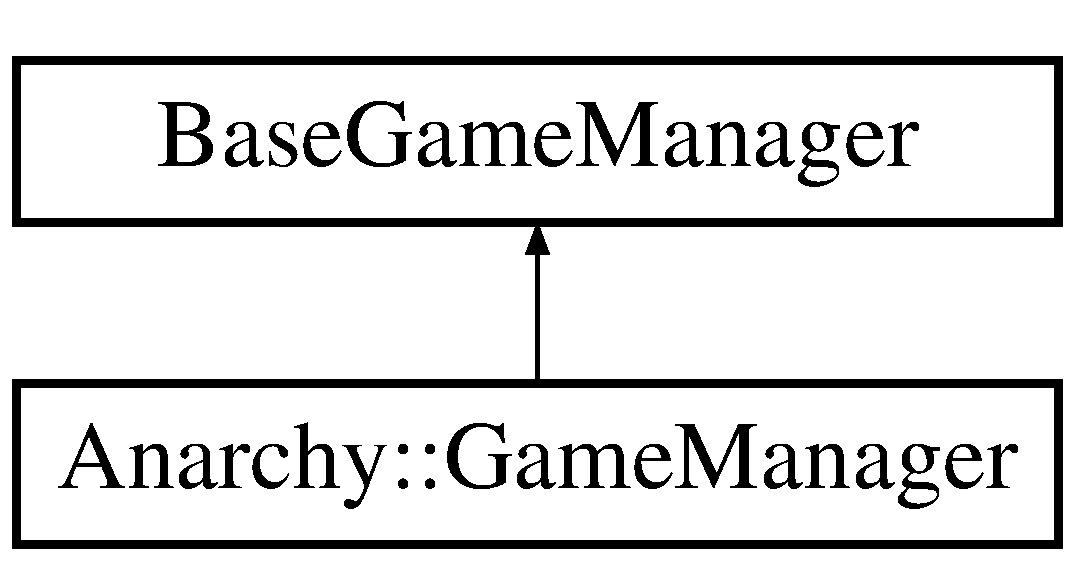
\includegraphics[height=2.000000cm]{classAnarchy_1_1GameManager}
\end{center}
\end{figure}
\subsection*{Public Member Functions}
\begin{DoxyCompactItemize}
\item 
\hypertarget{classAnarchy_1_1GameManager_a2c0754340cb44a6f84afdd92dbf85d08}{void {\bfseries setup\-A\-I} (const std\-::string \&player\-I\-D)}\label{classAnarchy_1_1GameManager_a2c0754340cb44a6f84afdd92dbf85d08}

\item 
\hypertarget{classAnarchy_1_1GameManager_a77f7032331fb9326b5cf6ab6e8a232e4}{boost\-::property\-\_\-tree\-::ptree $\ast$ {\bfseries order\-A\-I} (const std\-::string \&order, boost\-::property\-\_\-tree\-::ptree $\ast$args)}\label{classAnarchy_1_1GameManager_a77f7032331fb9326b5cf6ab6e8a232e4}

\end{DoxyCompactItemize}


\subsection{Detailed Description}
This is a class that manages the Anarchy \hyperlink{classAnarchy_1_1Game}{Game} and it's Game\-Objects. Competitors should never have to care about this class's existance. 



The documentation for this class was generated from the following files\-:\begin{DoxyCompactItemize}
\item 
game\-Manager.\-h\item 
game\-Manager.\-cpp\end{DoxyCompactItemize}

\hypertarget{classAnarchy_1_1GameObject}{\section{Anarchy\-:\-:Game\-Object Class Reference}
\label{classAnarchy_1_1GameObject}\index{Anarchy\-::\-Game\-Object@{Anarchy\-::\-Game\-Object}}
}


An object in the game. The most basic class that all game classes should inherit from automatically.  




{\ttfamily \#include $<$game\-Object.\-h$>$}

Inheritance diagram for Anarchy\-:\-:Game\-Object\-:\begin{figure}[H]
\begin{center}
\leavevmode
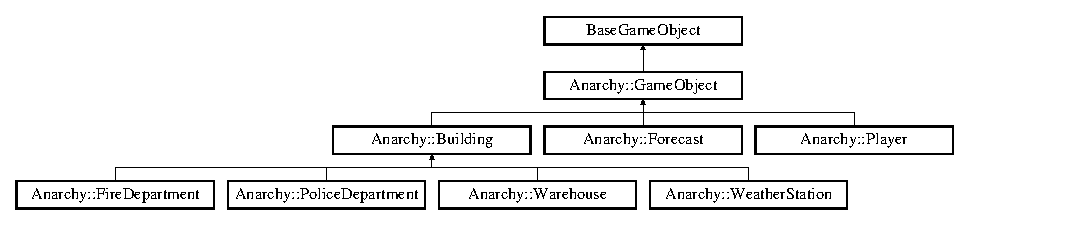
\includegraphics[height=2.574713cm]{classAnarchy_1_1GameObject}
\end{center}
\end{figure}
\subsection*{Public Member Functions}
\begin{DoxyCompactItemize}
\item 
void \hyperlink{classAnarchy_1_1GameObject_a962246ccd2b9ecf15478a9b46e6340fb}{log} (std\-::string message)
\begin{DoxyCompactList}\small\item\em adds a message to this game object's log. Intended for debugging purposes. \end{DoxyCompactList}\end{DoxyCompactItemize}
\subsection*{Public Attributes}
\begin{DoxyCompactItemize}
\item 
std\-::vector$<$ std\-::string $>$ \hyperlink{classAnarchy_1_1GameObject_ac1d185992a4219a51e1d1d5f71114567}{logs}
\begin{DoxyCompactList}\small\item\em Any strings logged will be stored here when this game object logs the strings. Intended for debugging. \end{DoxyCompactList}\end{DoxyCompactItemize}
\subsection*{Protected Member Functions}
\begin{DoxyCompactItemize}
\item 
\hypertarget{classAnarchy_1_1GameObject_a95283cfa759dbf3a88c6d87fc426bdce}{virtual void {\bfseries delta\-Update\-Field} (const std\-::string \&field\-Name, boost\-::property\-\_\-tree\-::ptree \&delta)}\label{classAnarchy_1_1GameObject_a95283cfa759dbf3a88c6d87fc426bdce}

\end{DoxyCompactItemize}


\subsection{Detailed Description}
An object in the game. The most basic class that all game classes should inherit from automatically. 



\subsection{Member Function Documentation}
\hypertarget{classAnarchy_1_1GameObject_a962246ccd2b9ecf15478a9b46e6340fb}{\index{Anarchy\-::\-Game\-Object@{Anarchy\-::\-Game\-Object}!log@{log}}
\index{log@{log}!Anarchy::GameObject@{Anarchy\-::\-Game\-Object}}
\subsubsection[{log}]{\setlength{\rightskip}{0pt plus 5cm}void Anarchy\-::\-Game\-Object\-::log (
\begin{DoxyParamCaption}
\item[{std\-::string}]{message}
\end{DoxyParamCaption}
)}}\label{classAnarchy_1_1GameObject_a962246ccd2b9ecf15478a9b46e6340fb}


adds a message to this game object's log. Intended for debugging purposes. 


\begin{DoxyParams}{Parameters}
{\em message} & A string to add to this \hyperlink{classAnarchy_1_1GameObject}{Game\-Object}'s log. Intended for debugging.\\
\hline
\end{DoxyParams}


\subsection{Member Data Documentation}
\hypertarget{classAnarchy_1_1GameObject_ac1d185992a4219a51e1d1d5f71114567}{\index{Anarchy\-::\-Game\-Object@{Anarchy\-::\-Game\-Object}!logs@{logs}}
\index{logs@{logs}!Anarchy::GameObject@{Anarchy\-::\-Game\-Object}}
\subsubsection[{logs}]{\setlength{\rightskip}{0pt plus 5cm}std\-::vector$<$std\-::string$>$ Anarchy\-::\-Game\-Object\-::logs}}\label{classAnarchy_1_1GameObject_ac1d185992a4219a51e1d1d5f71114567}


Any strings logged will be stored here when this game object logs the strings. Intended for debugging. 



The documentation for this class was generated from the following files\-:\begin{DoxyCompactItemize}
\item 
game\-Object.\-h\item 
game\-Object.\-cpp\end{DoxyCompactItemize}

\hypertarget{classAnarchy_1_1Player}{\section{Anarchy\-:\-:Player Class Reference}
\label{classAnarchy_1_1Player}\index{Anarchy\-::\-Player@{Anarchy\-::\-Player}}
}


A player in this game. Every \hyperlink{classAnarchy_1_1AI}{A\-I} controls one player.  




{\ttfamily \#include $<$player.\-h$>$}

Inheritance diagram for Anarchy\-:\-:Player\-:\begin{figure}[H]
\begin{center}
\leavevmode
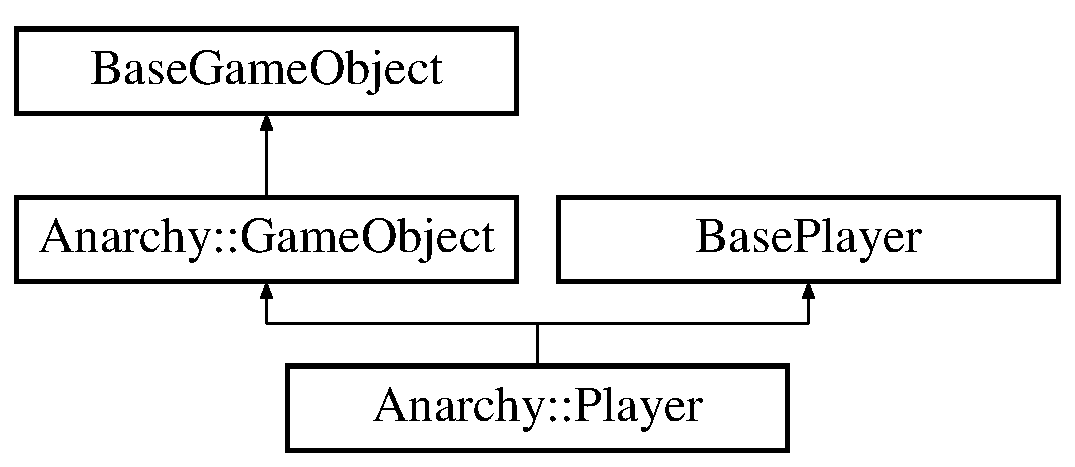
\includegraphics[height=3.000000cm]{classAnarchy_1_1Player}
\end{center}
\end{figure}
\subsection*{Public Attributes}
\begin{DoxyCompactItemize}
\item 
int \hyperlink{classAnarchy_1_1Player_a439ac9bc65f337358c0169f6352a3336}{bribes\-Remaining}
\begin{DoxyCompactList}\small\item\em How many bribes this player has remaining to use during their turn. Each action a \hyperlink{classAnarchy_1_1Building}{Building} does costs 1 bribe. Any unused bribes are lost at the end of the player's turn. \end{DoxyCompactList}\item 
std\-::vector$<$ \hyperlink{classAnarchy_1_1Building}{Anarchy\-::\-Building} $\ast$ $>$ \hyperlink{classAnarchy_1_1Player_a2b80bb75995c73f78df64ca6241cbc7b}{buildings}
\begin{DoxyCompactList}\small\item\em All the buildings owned by this player. \end{DoxyCompactList}\item 
std\-::string \hyperlink{classAnarchy_1_1Player_af5b7bce5d4d05b69d8b83d095f3ab39e}{client\-Type}
\begin{DoxyCompactList}\small\item\em What type of client this is, e.\-g. 'Python', 'Java\-Script', or some other language. For potential data mining purposes. \end{DoxyCompactList}\item 
std\-::vector\\*
$<$ \hyperlink{classAnarchy_1_1FireDepartment}{Anarchy\-::\-Fire\-Department} $\ast$ $>$ \hyperlink{classAnarchy_1_1Player_a9ef8ddd89632fa942b09c5d5f47d432c}{fire\-Departments}
\begin{DoxyCompactList}\small\item\em All the Fire\-Departments owned by this player. \end{DoxyCompactList}\item 
\hyperlink{classAnarchy_1_1Warehouse}{Anarchy\-::\-Warehouse} $\ast$ \hyperlink{classAnarchy_1_1Player_a175881daf024ff4b2ed8b7b7d0a8ab6b}{headquarters}
\begin{DoxyCompactList}\small\item\em The \hyperlink{classAnarchy_1_1Warehouse}{Warehouse} that serves as this player's headquarters and has extra health. If this gets destroyed they lose. \end{DoxyCompactList}\item 
std\-::string \hyperlink{classAnarchy_1_1Player_aafaac857aee9c030ae5908678eef613d}{name}
\begin{DoxyCompactList}\small\item\em The name of the player \end{DoxyCompactList}\item 
\hyperlink{classAnarchy_1_1Player}{Anarchy\-::\-Player} $\ast$ \hyperlink{classAnarchy_1_1Player_aa2cc74a91a193fb6ec24e28b3c78e2df}{other\-Player}
\begin{DoxyCompactList}\small\item\em this player's opponent in the game. \end{DoxyCompactList}\item 
std\-::vector\\*
$<$ \hyperlink{classAnarchy_1_1PoliceDepartment}{Anarchy\-::\-Police\-Department} $\ast$ $>$ \hyperlink{classAnarchy_1_1Player_a92ae92a6a0f6a491ec4ed9cd20cc598e}{police\-Departments}
\begin{DoxyCompactList}\small\item\em All the Police\-Departments owned by this player. \end{DoxyCompactList}\item 
float \hyperlink{classAnarchy_1_1Player_a242266d4bd3c79253b01173be7db0db9}{time\-Remaining}
\begin{DoxyCompactList}\small\item\em The amount of time (in ns) remaining for this \hyperlink{classAnarchy_1_1AI}{A\-I} to send commands. \end{DoxyCompactList}\item 
std\-::vector$<$ \hyperlink{classAnarchy_1_1Warehouse}{Anarchy\-::\-Warehouse} $\ast$ $>$ \hyperlink{classAnarchy_1_1Player_ae2913affe60c619b4b7d25475f677804}{warehouses}
\begin{DoxyCompactList}\small\item\em All the warehouses owned by this player. Includes the Headquarters. \end{DoxyCompactList}\item 
std\-::vector\\*
$<$ \hyperlink{classAnarchy_1_1WeatherStation}{Anarchy\-::\-Weather\-Station} $\ast$ $>$ \hyperlink{classAnarchy_1_1Player_a7738ef75a6b23b3d48a7b6084a21c59c}{weather\-Stations}
\begin{DoxyCompactList}\small\item\em All the Weather\-Stations owned by this player. \end{DoxyCompactList}\end{DoxyCompactItemize}
\subsection*{Protected Member Functions}
\begin{DoxyCompactItemize}
\item 
\hypertarget{classAnarchy_1_1Player_a4a8fd3162e3a6eba89b48348c346c0c7}{virtual void {\bfseries delta\-Update\-Field} (const std\-::string \&field\-Name, boost\-::property\-\_\-tree\-::ptree \&delta)}\label{classAnarchy_1_1Player_a4a8fd3162e3a6eba89b48348c346c0c7}

\end{DoxyCompactItemize}
\subsection*{Additional Inherited Members}


\subsection{Detailed Description}
A player in this game. Every \hyperlink{classAnarchy_1_1AI}{A\-I} controls one player. 



\subsection{Member Data Documentation}
\hypertarget{classAnarchy_1_1Player_a439ac9bc65f337358c0169f6352a3336}{\index{Anarchy\-::\-Player@{Anarchy\-::\-Player}!bribes\-Remaining@{bribes\-Remaining}}
\index{bribes\-Remaining@{bribes\-Remaining}!Anarchy::Player@{Anarchy\-::\-Player}}
\subsubsection[{bribes\-Remaining}]{\setlength{\rightskip}{0pt plus 5cm}int Anarchy\-::\-Player\-::bribes\-Remaining}}\label{classAnarchy_1_1Player_a439ac9bc65f337358c0169f6352a3336}


How many bribes this player has remaining to use during their turn. Each action a \hyperlink{classAnarchy_1_1Building}{Building} does costs 1 bribe. Any unused bribes are lost at the end of the player's turn. 

\hypertarget{classAnarchy_1_1Player_a2b80bb75995c73f78df64ca6241cbc7b}{\index{Anarchy\-::\-Player@{Anarchy\-::\-Player}!buildings@{buildings}}
\index{buildings@{buildings}!Anarchy::Player@{Anarchy\-::\-Player}}
\subsubsection[{buildings}]{\setlength{\rightskip}{0pt plus 5cm}std\-::vector$<${\bf Anarchy\-::\-Building}$\ast$$>$ Anarchy\-::\-Player\-::buildings}}\label{classAnarchy_1_1Player_a2b80bb75995c73f78df64ca6241cbc7b}


All the buildings owned by this player. 

\hypertarget{classAnarchy_1_1Player_af5b7bce5d4d05b69d8b83d095f3ab39e}{\index{Anarchy\-::\-Player@{Anarchy\-::\-Player}!client\-Type@{client\-Type}}
\index{client\-Type@{client\-Type}!Anarchy::Player@{Anarchy\-::\-Player}}
\subsubsection[{client\-Type}]{\setlength{\rightskip}{0pt plus 5cm}std\-::string Anarchy\-::\-Player\-::client\-Type}}\label{classAnarchy_1_1Player_af5b7bce5d4d05b69d8b83d095f3ab39e}


What type of client this is, e.\-g. 'Python', 'Java\-Script', or some other language. For potential data mining purposes. 

\hypertarget{classAnarchy_1_1Player_a9ef8ddd89632fa942b09c5d5f47d432c}{\index{Anarchy\-::\-Player@{Anarchy\-::\-Player}!fire\-Departments@{fire\-Departments}}
\index{fire\-Departments@{fire\-Departments}!Anarchy::Player@{Anarchy\-::\-Player}}
\subsubsection[{fire\-Departments}]{\setlength{\rightskip}{0pt plus 5cm}std\-::vector$<${\bf Anarchy\-::\-Fire\-Department}$\ast$$>$ Anarchy\-::\-Player\-::fire\-Departments}}\label{classAnarchy_1_1Player_a9ef8ddd89632fa942b09c5d5f47d432c}


All the Fire\-Departments owned by this player. 

\hypertarget{classAnarchy_1_1Player_a175881daf024ff4b2ed8b7b7d0a8ab6b}{\index{Anarchy\-::\-Player@{Anarchy\-::\-Player}!headquarters@{headquarters}}
\index{headquarters@{headquarters}!Anarchy::Player@{Anarchy\-::\-Player}}
\subsubsection[{headquarters}]{\setlength{\rightskip}{0pt plus 5cm}{\bf Anarchy\-::\-Warehouse}$\ast$ Anarchy\-::\-Player\-::headquarters}}\label{classAnarchy_1_1Player_a175881daf024ff4b2ed8b7b7d0a8ab6b}


The \hyperlink{classAnarchy_1_1Warehouse}{Warehouse} that serves as this player's headquarters and has extra health. If this gets destroyed they lose. 

\hypertarget{classAnarchy_1_1Player_aafaac857aee9c030ae5908678eef613d}{\index{Anarchy\-::\-Player@{Anarchy\-::\-Player}!name@{name}}
\index{name@{name}!Anarchy::Player@{Anarchy\-::\-Player}}
\subsubsection[{name}]{\setlength{\rightskip}{0pt plus 5cm}std\-::string Anarchy\-::\-Player\-::name}}\label{classAnarchy_1_1Player_aafaac857aee9c030ae5908678eef613d}


The name of the player 

\hypertarget{classAnarchy_1_1Player_aa2cc74a91a193fb6ec24e28b3c78e2df}{\index{Anarchy\-::\-Player@{Anarchy\-::\-Player}!other\-Player@{other\-Player}}
\index{other\-Player@{other\-Player}!Anarchy::Player@{Anarchy\-::\-Player}}
\subsubsection[{other\-Player}]{\setlength{\rightskip}{0pt plus 5cm}{\bf Anarchy\-::\-Player}$\ast$ Anarchy\-::\-Player\-::other\-Player}}\label{classAnarchy_1_1Player_aa2cc74a91a193fb6ec24e28b3c78e2df}


this player's opponent in the game. 

\hypertarget{classAnarchy_1_1Player_a92ae92a6a0f6a491ec4ed9cd20cc598e}{\index{Anarchy\-::\-Player@{Anarchy\-::\-Player}!police\-Departments@{police\-Departments}}
\index{police\-Departments@{police\-Departments}!Anarchy::Player@{Anarchy\-::\-Player}}
\subsubsection[{police\-Departments}]{\setlength{\rightskip}{0pt plus 5cm}std\-::vector$<${\bf Anarchy\-::\-Police\-Department}$\ast$$>$ Anarchy\-::\-Player\-::police\-Departments}}\label{classAnarchy_1_1Player_a92ae92a6a0f6a491ec4ed9cd20cc598e}


All the Police\-Departments owned by this player. 

\hypertarget{classAnarchy_1_1Player_a242266d4bd3c79253b01173be7db0db9}{\index{Anarchy\-::\-Player@{Anarchy\-::\-Player}!time\-Remaining@{time\-Remaining}}
\index{time\-Remaining@{time\-Remaining}!Anarchy::Player@{Anarchy\-::\-Player}}
\subsubsection[{time\-Remaining}]{\setlength{\rightskip}{0pt plus 5cm}float Anarchy\-::\-Player\-::time\-Remaining}}\label{classAnarchy_1_1Player_a242266d4bd3c79253b01173be7db0db9}


The amount of time (in ns) remaining for this \hyperlink{classAnarchy_1_1AI}{A\-I} to send commands. 

\hypertarget{classAnarchy_1_1Player_ae2913affe60c619b4b7d25475f677804}{\index{Anarchy\-::\-Player@{Anarchy\-::\-Player}!warehouses@{warehouses}}
\index{warehouses@{warehouses}!Anarchy::Player@{Anarchy\-::\-Player}}
\subsubsection[{warehouses}]{\setlength{\rightskip}{0pt plus 5cm}std\-::vector$<${\bf Anarchy\-::\-Warehouse}$\ast$$>$ Anarchy\-::\-Player\-::warehouses}}\label{classAnarchy_1_1Player_ae2913affe60c619b4b7d25475f677804}


All the warehouses owned by this player. Includes the Headquarters. 

\hypertarget{classAnarchy_1_1Player_a7738ef75a6b23b3d48a7b6084a21c59c}{\index{Anarchy\-::\-Player@{Anarchy\-::\-Player}!weather\-Stations@{weather\-Stations}}
\index{weather\-Stations@{weather\-Stations}!Anarchy::Player@{Anarchy\-::\-Player}}
\subsubsection[{weather\-Stations}]{\setlength{\rightskip}{0pt plus 5cm}std\-::vector$<${\bf Anarchy\-::\-Weather\-Station}$\ast$$>$ Anarchy\-::\-Player\-::weather\-Stations}}\label{classAnarchy_1_1Player_a7738ef75a6b23b3d48a7b6084a21c59c}


All the Weather\-Stations owned by this player. 



The documentation for this class was generated from the following files\-:\begin{DoxyCompactItemize}
\item 
player.\-h\item 
player.\-cpp\end{DoxyCompactItemize}

\hypertarget{classAnarchy_1_1PoliceDepartment}{\section{Anarchy\-:\-:Police\-Department Class Reference}
\label{classAnarchy_1_1PoliceDepartment}\index{Anarchy\-::\-Police\-Department@{Anarchy\-::\-Police\-Department}}
}


Used to keep cities under control and raid Warehouses.  




{\ttfamily \#include $<$police\-Department.\-h$>$}

Inheritance diagram for Anarchy\-:\-:Police\-Department\-:\begin{figure}[H]
\begin{center}
\leavevmode
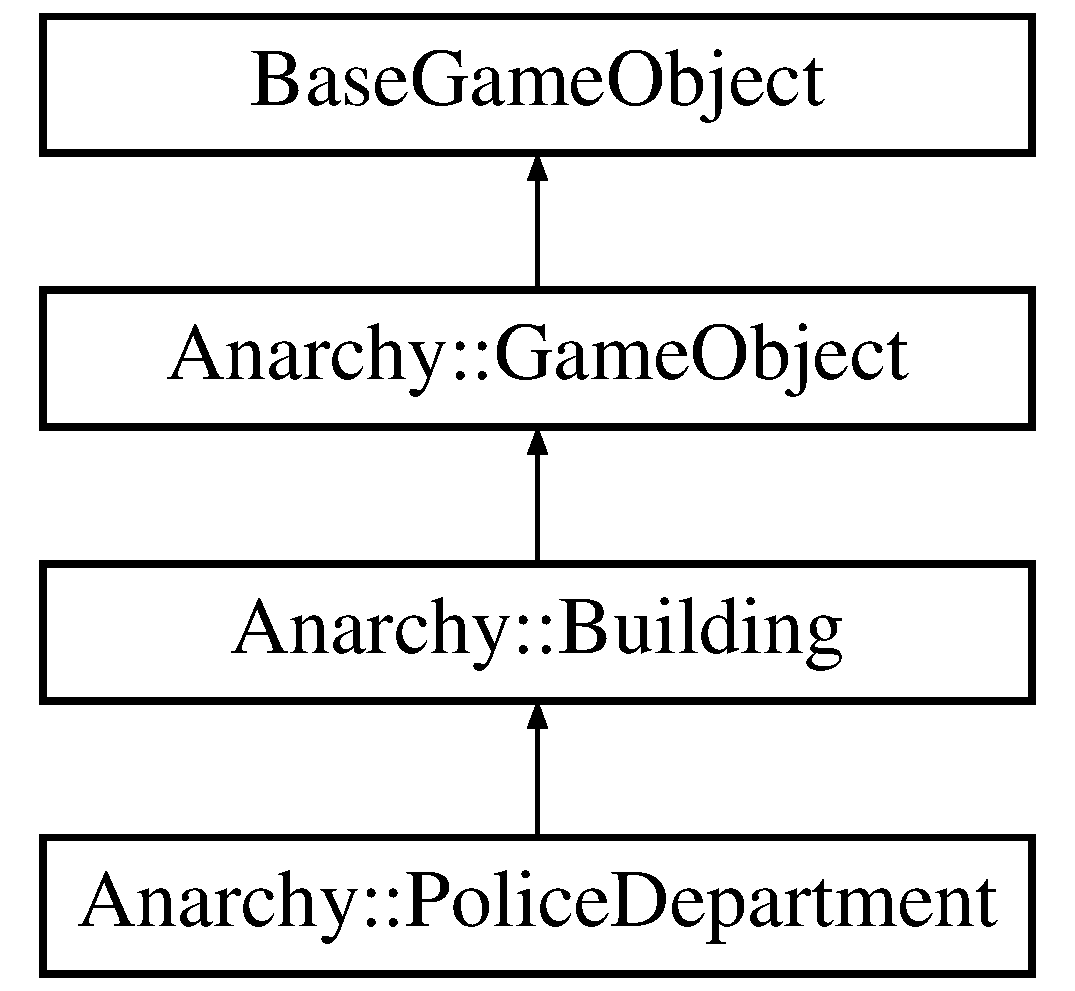
\includegraphics[height=4.000000cm]{classAnarchy_1_1PoliceDepartment}
\end{center}
\end{figure}
\subsection*{Public Member Functions}
\begin{DoxyCompactItemize}
\item 
int \hyperlink{classAnarchy_1_1PoliceDepartment_a88ac84ac3faad7d8f34cd2ec77805272}{raid} (\hyperlink{classAnarchy_1_1Warehouse}{Anarchy\-::\-Warehouse} $\ast$warehouse)
\begin{DoxyCompactList}\small\item\em Bribe the police to raid a \hyperlink{classAnarchy_1_1Warehouse}{Warehouse}, dealing damage equal based on the \hyperlink{classAnarchy_1_1Warehouse}{Warehouse}'s current exposure, and then resetting it to 0. \end{DoxyCompactList}\end{DoxyCompactItemize}
\subsection*{Protected Member Functions}
\begin{DoxyCompactItemize}
\item 
\hypertarget{classAnarchy_1_1PoliceDepartment_a6103f32d50ebfa747a5c77fdd476136c}{virtual void {\bfseries delta\-Update\-Field} (const std\-::string \&field\-Name, boost\-::property\-\_\-tree\-::ptree \&delta)}\label{classAnarchy_1_1PoliceDepartment_a6103f32d50ebfa747a5c77fdd476136c}

\end{DoxyCompactItemize}
\subsection*{Additional Inherited Members}


\subsection{Detailed Description}
Used to keep cities under control and raid Warehouses. 



\subsection{Member Function Documentation}
\hypertarget{classAnarchy_1_1PoliceDepartment_a88ac84ac3faad7d8f34cd2ec77805272}{\index{Anarchy\-::\-Police\-Department@{Anarchy\-::\-Police\-Department}!raid@{raid}}
\index{raid@{raid}!Anarchy::PoliceDepartment@{Anarchy\-::\-Police\-Department}}
\subsubsection[{raid}]{\setlength{\rightskip}{0pt plus 5cm}int Anarchy\-::\-Police\-Department\-::raid (
\begin{DoxyParamCaption}
\item[{{\bf Anarchy\-::\-Warehouse} $\ast$}]{warehouse}
\end{DoxyParamCaption}
)}}\label{classAnarchy_1_1PoliceDepartment_a88ac84ac3faad7d8f34cd2ec77805272}


Bribe the police to raid a \hyperlink{classAnarchy_1_1Warehouse}{Warehouse}, dealing damage equal based on the \hyperlink{classAnarchy_1_1Warehouse}{Warehouse}'s current exposure, and then resetting it to 0. 


\begin{DoxyParams}{Parameters}
{\em warehouse} & The warehouse you want to raid.\\
\hline
\end{DoxyParams}
\begin{DoxyReturn}{Returns}
The amount of damage dealt to the warehouse, or -\/1 if there was an error.
\end{DoxyReturn}


The documentation for this class was generated from the following files\-:\begin{DoxyCompactItemize}
\item 
police\-Department.\-h\item 
police\-Department.\-cpp\end{DoxyCompactItemize}

\hypertarget{classAnarchy_1_1Warehouse}{\section{Anarchy\-:\-:Warehouse Class Reference}
\label{classAnarchy_1_1Warehouse}\index{Anarchy\-::\-Warehouse@{Anarchy\-::\-Warehouse}}
}


A typical abandoned warehouse... that anarchists hang out in and can be bribed to burn down Buildings.  




{\ttfamily \#include $<$warehouse.\-h$>$}

Inheritance diagram for Anarchy\-:\-:Warehouse\-:\begin{figure}[H]
\begin{center}
\leavevmode
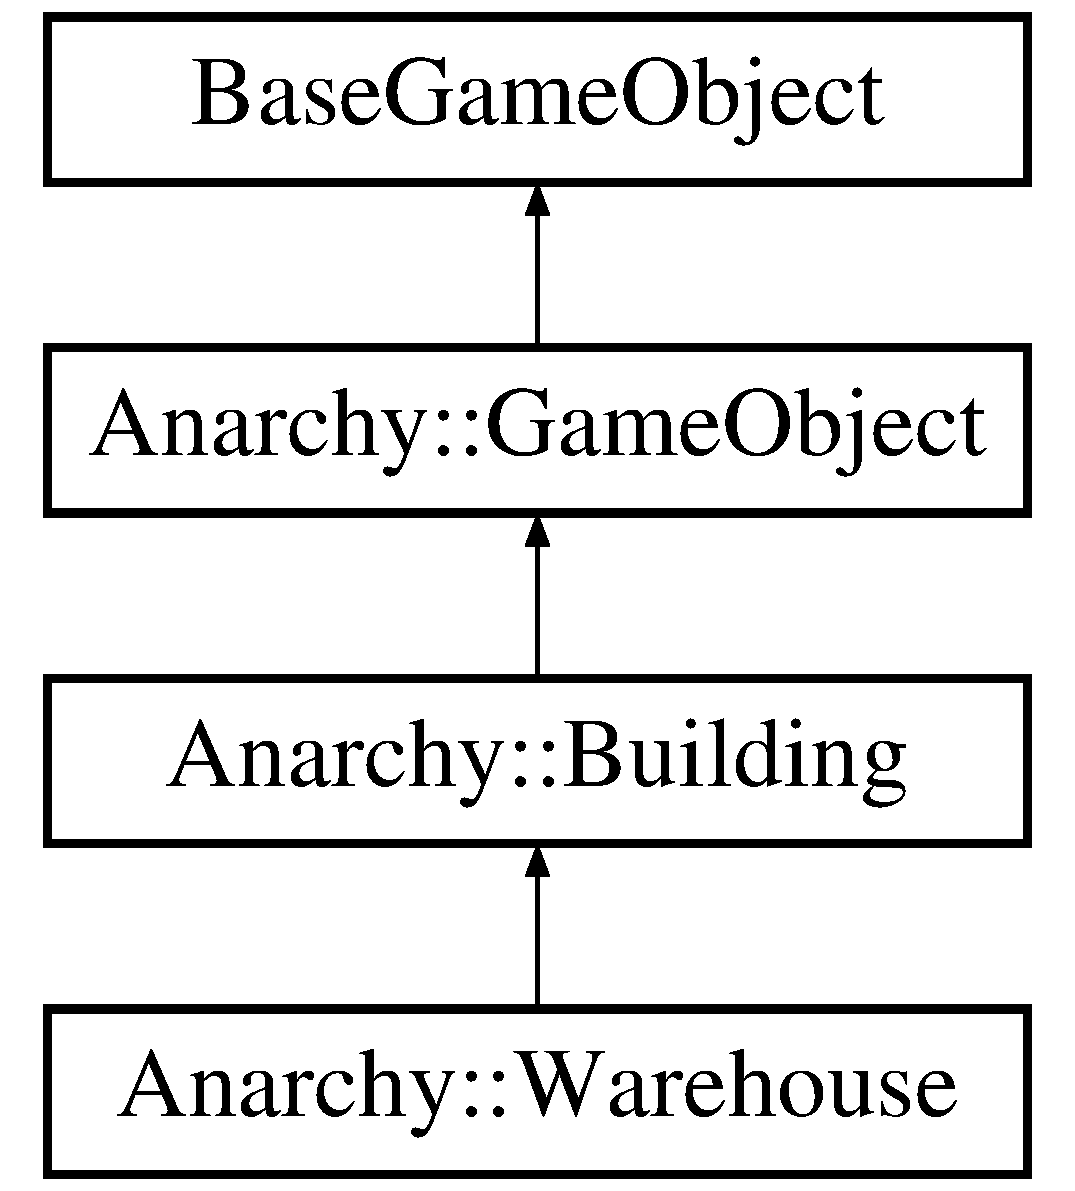
\includegraphics[height=4.000000cm]{classAnarchy_1_1Warehouse}
\end{center}
\end{figure}
\subsection*{Public Member Functions}
\begin{DoxyCompactItemize}
\item 
int \hyperlink{classAnarchy_1_1Warehouse_a8f6b4bb3e14832987703652dde82d6b7}{ignite} (\hyperlink{classAnarchy_1_1Building}{Anarchy\-::\-Building} $\ast$building)
\begin{DoxyCompactList}\small\item\em Bribes the \hyperlink{classAnarchy_1_1Warehouse}{Warehouse} to light a \hyperlink{classAnarchy_1_1Building}{Building} on fire. This adds this building's fire\-Added to their fire, and then this building's exposure is increased based on the Manhatten distance between the two buildings. \end{DoxyCompactList}\end{DoxyCompactItemize}
\subsection*{Public Attributes}
\begin{DoxyCompactItemize}
\item 
int \hyperlink{classAnarchy_1_1Warehouse_a98c01b33a1a27d2d2e47a33d3ed9dc06}{exposure}
\begin{DoxyCompactList}\small\item\em How exposed the anarchists in this warehouse are to Police\-Departments. Raises when bribed to ignite buildings, and drops each turn if not bribed. \end{DoxyCompactList}\item 
int \hyperlink{classAnarchy_1_1Warehouse_a646bc6f8bbd539ea88b9b68593b6f5b7}{fire\-Added}
\begin{DoxyCompactList}\small\item\em The amount of fire added to buildings when bribed to ignite a building. Headquarters add more fire than normal Warehouses. \end{DoxyCompactList}\end{DoxyCompactItemize}
\subsection*{Protected Member Functions}
\begin{DoxyCompactItemize}
\item 
\hypertarget{classAnarchy_1_1Warehouse_add5db92819e80df654425d36f1a75695}{virtual void {\bfseries delta\-Update\-Field} (const std\-::string \&field\-Name, boost\-::property\-\_\-tree\-::ptree \&delta)}\label{classAnarchy_1_1Warehouse_add5db92819e80df654425d36f1a75695}

\end{DoxyCompactItemize}


\subsection{Detailed Description}
A typical abandoned warehouse... that anarchists hang out in and can be bribed to burn down Buildings. 



\subsection{Member Function Documentation}
\hypertarget{classAnarchy_1_1Warehouse_a8f6b4bb3e14832987703652dde82d6b7}{\index{Anarchy\-::\-Warehouse@{Anarchy\-::\-Warehouse}!ignite@{ignite}}
\index{ignite@{ignite}!Anarchy::Warehouse@{Anarchy\-::\-Warehouse}}
\subsubsection[{ignite}]{\setlength{\rightskip}{0pt plus 5cm}int Anarchy\-::\-Warehouse\-::ignite (
\begin{DoxyParamCaption}
\item[{{\bf Anarchy\-::\-Building} $\ast$}]{building}
\end{DoxyParamCaption}
)}}\label{classAnarchy_1_1Warehouse_a8f6b4bb3e14832987703652dde82d6b7}


Bribes the \hyperlink{classAnarchy_1_1Warehouse}{Warehouse} to light a \hyperlink{classAnarchy_1_1Building}{Building} on fire. This adds this building's fire\-Added to their fire, and then this building's exposure is increased based on the Manhatten distance between the two buildings. 


\begin{DoxyParams}{Parameters}
{\em building} & The \hyperlink{classAnarchy_1_1Building}{Building} you want to light on fire.\\
\hline
\end{DoxyParams}
\begin{DoxyReturn}{Returns}
The exposure added to this \hyperlink{classAnarchy_1_1Building}{Building}'s exposure. -\/1 is returned if there was an error.
\end{DoxyReturn}


\subsection{Member Data Documentation}
\hypertarget{classAnarchy_1_1Warehouse_a98c01b33a1a27d2d2e47a33d3ed9dc06}{\index{Anarchy\-::\-Warehouse@{Anarchy\-::\-Warehouse}!exposure@{exposure}}
\index{exposure@{exposure}!Anarchy::Warehouse@{Anarchy\-::\-Warehouse}}
\subsubsection[{exposure}]{\setlength{\rightskip}{0pt plus 5cm}int Anarchy\-::\-Warehouse\-::exposure}}\label{classAnarchy_1_1Warehouse_a98c01b33a1a27d2d2e47a33d3ed9dc06}


How exposed the anarchists in this warehouse are to Police\-Departments. Raises when bribed to ignite buildings, and drops each turn if not bribed. 

\hypertarget{classAnarchy_1_1Warehouse_a646bc6f8bbd539ea88b9b68593b6f5b7}{\index{Anarchy\-::\-Warehouse@{Anarchy\-::\-Warehouse}!fire\-Added@{fire\-Added}}
\index{fire\-Added@{fire\-Added}!Anarchy::Warehouse@{Anarchy\-::\-Warehouse}}
\subsubsection[{fire\-Added}]{\setlength{\rightskip}{0pt plus 5cm}int Anarchy\-::\-Warehouse\-::fire\-Added}}\label{classAnarchy_1_1Warehouse_a646bc6f8bbd539ea88b9b68593b6f5b7}


The amount of fire added to buildings when bribed to ignite a building. Headquarters add more fire than normal Warehouses. 



The documentation for this class was generated from the following files\-:\begin{DoxyCompactItemize}
\item 
warehouse.\-h\item 
warehouse.\-cpp\end{DoxyCompactItemize}

\hypertarget{classAnarchy_1_1WeatherStation}{\section{Anarchy\-:\-:Weather\-Station Class Reference}
\label{classAnarchy_1_1WeatherStation}\index{Anarchy\-::\-Weather\-Station@{Anarchy\-::\-Weather\-Station}}
}


Can be bribed to change the next \hyperlink{classAnarchy_1_1Forecast}{Forecast} in some way.  




{\ttfamily \#include $<$weather\-Station.\-h$>$}

Inheritance diagram for Anarchy\-:\-:Weather\-Station\-:\begin{figure}[H]
\begin{center}
\leavevmode
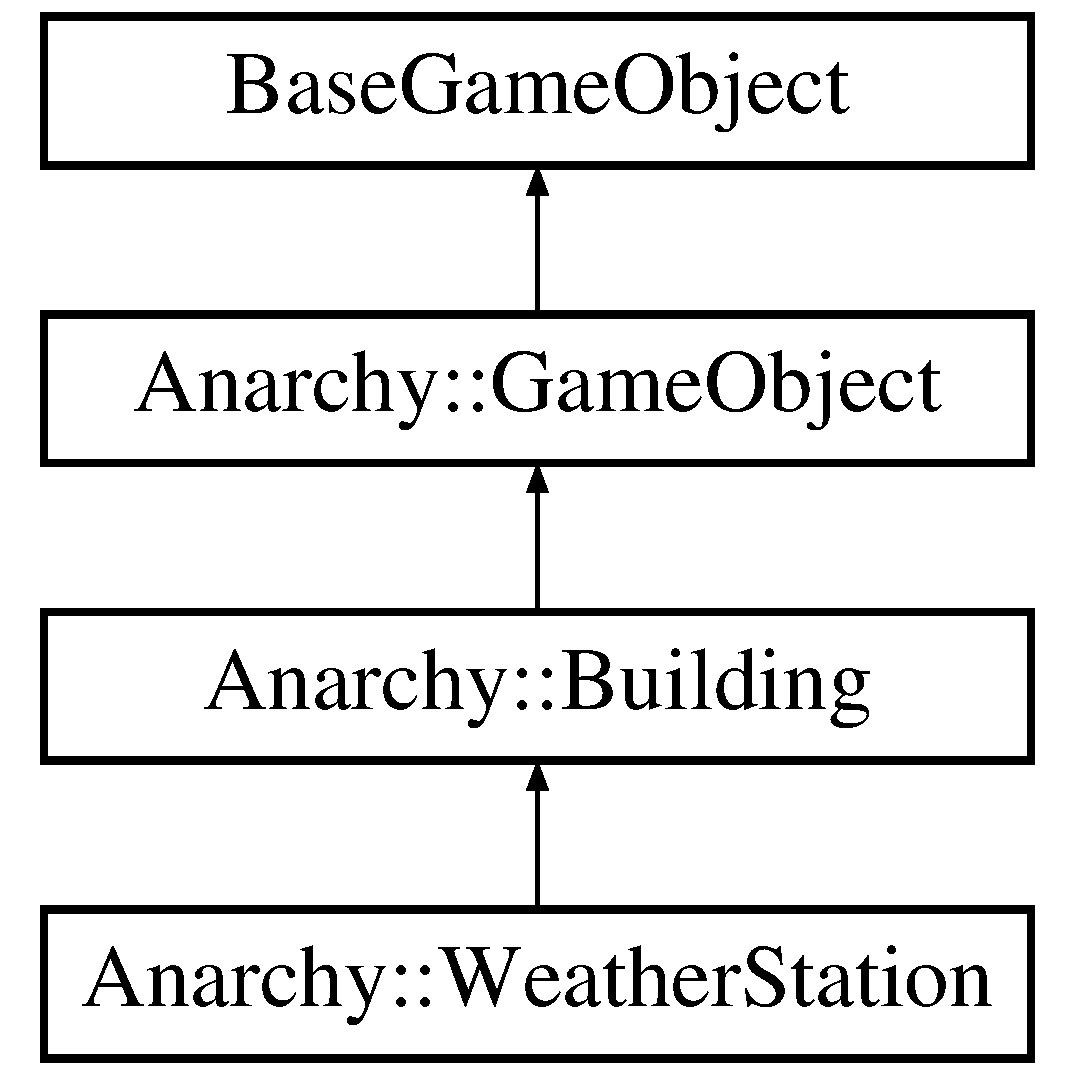
\includegraphics[height=4.000000cm]{classAnarchy_1_1WeatherStation}
\end{center}
\end{figure}
\subsection*{Public Member Functions}
\begin{DoxyCompactItemize}
\item 
bool \hyperlink{classAnarchy_1_1WeatherStation_aa1aee54cf7e190dcfbcbd46c893623df}{intensify} (bool negative=false)
\begin{DoxyCompactList}\small\item\em Bribe the weathermen to intensity the next \hyperlink{classAnarchy_1_1Forecast}{Forecast} by 1 or -\/1 \end{DoxyCompactList}\item 
bool \hyperlink{classAnarchy_1_1WeatherStation_a331b6a3cb2831fb40a9c0e083754ef78}{rotate} (bool counterclockwise=false)
\begin{DoxyCompactList}\small\item\em Bribe the weathermen to change the direction of the next \hyperlink{classAnarchy_1_1Forecast}{Forecast} by rotating it clockwise or counterclockwise. \end{DoxyCompactList}\end{DoxyCompactItemize}
\subsection*{Protected Member Functions}
\begin{DoxyCompactItemize}
\item 
\hypertarget{classAnarchy_1_1WeatherStation_a1e031e4c1809c3ada2266f8798a49740}{virtual void {\bfseries delta\-Update\-Field} (const std\-::string \&field\-Name, boost\-::property\-\_\-tree\-::ptree \&delta)}\label{classAnarchy_1_1WeatherStation_a1e031e4c1809c3ada2266f8798a49740}

\end{DoxyCompactItemize}
\subsection*{Additional Inherited Members}


\subsection{Detailed Description}
Can be bribed to change the next \hyperlink{classAnarchy_1_1Forecast}{Forecast} in some way. 



\subsection{Member Function Documentation}
\hypertarget{classAnarchy_1_1WeatherStation_aa1aee54cf7e190dcfbcbd46c893623df}{\index{Anarchy\-::\-Weather\-Station@{Anarchy\-::\-Weather\-Station}!intensify@{intensify}}
\index{intensify@{intensify}!Anarchy::WeatherStation@{Anarchy\-::\-Weather\-Station}}
\subsubsection[{intensify}]{\setlength{\rightskip}{0pt plus 5cm}bool Anarchy\-::\-Weather\-Station\-::intensify (
\begin{DoxyParamCaption}
\item[{bool}]{negative = {\ttfamily false}}
\end{DoxyParamCaption}
)}}\label{classAnarchy_1_1WeatherStation_aa1aee54cf7e190dcfbcbd46c893623df}


Bribe the weathermen to intensity the next \hyperlink{classAnarchy_1_1Forecast}{Forecast} by 1 or -\/1 


\begin{DoxyParams}{Parameters}
{\em negative} & By default the intensity will be increased by 1, setting this to true decreases the intensity by 1.\\
\hline
\end{DoxyParams}
\begin{DoxyReturn}{Returns}
true if the intensity was changed, false otherwise
\end{DoxyReturn}
\hypertarget{classAnarchy_1_1WeatherStation_a331b6a3cb2831fb40a9c0e083754ef78}{\index{Anarchy\-::\-Weather\-Station@{Anarchy\-::\-Weather\-Station}!rotate@{rotate}}
\index{rotate@{rotate}!Anarchy::WeatherStation@{Anarchy\-::\-Weather\-Station}}
\subsubsection[{rotate}]{\setlength{\rightskip}{0pt plus 5cm}bool Anarchy\-::\-Weather\-Station\-::rotate (
\begin{DoxyParamCaption}
\item[{bool}]{counterclockwise = {\ttfamily false}}
\end{DoxyParamCaption}
)}}\label{classAnarchy_1_1WeatherStation_a331b6a3cb2831fb40a9c0e083754ef78}


Bribe the weathermen to change the direction of the next \hyperlink{classAnarchy_1_1Forecast}{Forecast} by rotating it clockwise or counterclockwise. 


\begin{DoxyParams}{Parameters}
{\em counterclockwise} & By default the direction will be rotated clockwise. If you set this to true we will rotate the forecast counterclockwise instead.\\
\hline
\end{DoxyParams}
\begin{DoxyReturn}{Returns}
true if the rotation worked, false otherwise.
\end{DoxyReturn}


The documentation for this class was generated from the following files\-:\begin{DoxyCompactItemize}
\item 
weather\-Station.\-h\item 
weather\-Station.\-cpp\end{DoxyCompactItemize}

%--- End generated contents ---

% Index
\newpage
\phantomsection
\addcontentsline{toc}{chapter}{Index}
\printindex

\end{document}
